\documentclass[conference]{IEEEtran}

% ---------- Math / Algo / Figures ----------
\usepackage{amsmath,amssymb,amsfonts,amsthm}
\usepackage{algorithm}
\usepackage{algpseudocode}
\usepackage{graphicx}
\graphicspath{{figures/}}
\usepackage{booktabs}
\usepackage{multirow}
\usepackage{placeins}
\usepackage{threeparttable}
\usepackage{tabularx}
\usepackage{array}
\usepackage{enumerate}
\usepackage{siunitx}


% ---------- Symbols ----------
\usepackage{pifont}
\newcommand{\cmark}{\ding{51}}  % ✓
\newcommand{\xmark}{\ding{55}}  % ✗
\newcolumntype{Y}{>{\raggedright\arraybackslash}X}

% ---------- Text / Utils ----------
\usepackage{times}
\DeclareFontShape{OT1}{ptm}{m}{scit}{<->ssub * ptm/m/sc}{}
\emergencystretch=3em
\hfuzz=500pt
\hbadness=10000
\vbadness=10000
\usepackage{soul}
\usepackage{url}
\usepackage{xcolor}
\usepackage[switch]{lineno}
\usepackage{xr}

\theoremstyle{definition}
\newtheorem{definition}{Definition}
\newtheorem{challenge}{Challenge}
% ---------- Biblatex (IMPORTANT) ----------
% 建议加 csquotes；biblatex 在某些环境下会提示它
\usepackage{csquotes}
\usepackage[backend=biber,style=ieee,sorting=none,sortcites=false]{biblatex}
\addbibresource{reference.bib}

% ---------- Hyperref should be near the end ----------
\usepackage[hidelinks]{hyperref}
\theoremstyle{plain}
\newtheorem{theorem}{Theorem}
\newtheorem{lemma}{Lemma}
\newtheorem{proposition}{Proposition}
\begin{document}

\title{TSIP: Proof-Carrying Continuity for Privacy-Preserving Location Aggregation}


% author names and affiliations
% use a multiple column layout for up to three different
% affiliations
\author{\IEEEauthorblockN{[Author names removed for blind review]}
	\IEEEauthorblockA{[Affiliation removed for blind review]}}
\maketitle
\begin{abstract}
Privacy-preserving location aggregation pipelines produce heatmaps that are
private but not necessarily truthful: existing designs validate each submission
in isolation and therefore admit cross-round attacks---teleportation, replay,
identity-swap, and gradual drift---whose trajectories are physically implausible
yet whose per-round predicates all pass.
We present \textsc{TSIP}, the first in-circuit enforcement of cross-round
trajectory continuity within an Encode-Shuffle-Analyze (ESA) private
aggregation pipeline.
Each client submission carries a 128-byte Groth16 proof that chains the new
location commitment to its predecessor and simultaneously enforces two
complementary constraints: a per-step speed bound and an
\emph{Anchor-Distance Window Continuity} (ADWC) constraint that bounds
$K$-round cumulative drift against a committed anchor.
The ADWC policy cap is exposed as a public input, enabling auditable
runtime tuning without re-running trusted setup; the proof sits upstream
of secure aggregation and leaves the downstream differentially private
release layer unchanged. On T-Drive and GeoLife with up to $1{,}000$ simulated clients, \textsc{TSIP}
detects $100\%$ of teleportation, replay, and identity-swap attacks at zero
circuit-level false rejects on benign traces, while preserving the utility
profile of a pure $\varepsilon{=}1.0$ differentially private release.
Proof generation takes ${\approx}\SI{0.34}{\second}$--${\approx}\SI{0.36}{\second}$
on a commodity CPU and per-submission communication is
${\approx}2$\,KB---practical for per-minute mobile submission rates.
The principal remaining limitation is the \emph{enrollment truth gap}:
\textsc{TSIP} guarantees continuity from a committed genesis point but
cannot cryptographically verify that the genesis itself is honest; the
Groth16 trusted-setup assumption also applies.
\end{abstract}
\IEEEpeerreviewmaketitle

% =============================================================
%  Introduction
%  Target venue: NDSS
% =============================================================

\section{Introduction}
\label{sec:intro}

Location heatmaps derived from mobile trajectories have become a core
primitive for modern urban computing.
Traffic engineering, public transit planning, and
environmental sensing all rely on population-level spatial statistics,
while individual raw coordinates must remain hidden from the
infrastructure~\cite{Zheng2010GeoLife,Yuan2010Tdrive}.
To meet this requirement, privacy-preserving location analytics systems
typically combine local differential privacy
(LDP)~\cite{Dwork2006calibrating,Andres2013geoi} with cryptographic secure
aggregation~\cite{Roth2019Nebula,Segal2017PracticalSecAgg}.
Substantial progress has therefore been made on the privacy--utility
trade-off of released heatmaps.

\begin{figure}[t]
  \centering
  \includegraphics[width=\columnwidth]{figures/attacking example.pdf}
  \caption{Two representative cross-round trajectory attacks on
    federated location aggregation.}
  \label{fig:example}
\end{figure}

Consider a city-scale mobility analytics platform that ingests anonymous
location signals from tens of thousands of smartphones to produce
real-time transit demand maps used for bus dispatching.
In such a deployment, each device submits a differentially privatised
report to an Encode-Shuffle-Analyze (ESA)
pipeline~\cite{Bittau2017Prochlo,Cheu2019distributed}: the shuffler
unlinks each report from its sender before the aggregator tallies cell
counts, so individual privacy is protected.
Per-round input validation can additionally be enforced via short
zero-knowledge proofs~\cite{Pillutla2024RiseFL,Chowdhury2022EIFFeL},
ensuring each submitted report satisfies a well-formed predicate
(e.g.\ the encoded cell index is in-range).
Yet neither the shuffle nor the per-round proof says anything about the
\emph{sequence} of reports a device submits over time.
A GPS-spoofing adversary---or a botnet of compromised handsets---can
submit reports that each pass every per-round check, while collectively
implying that a single ``user'' commuted 50\,km in three minutes,
reappeared at a distant transit hub it last visited six hours ago, or
simultaneously contributed to two geographically separated cells.
The corrupted aggregate silently redirects buses to artificially inflated
demand points, degrades the utility of downstream differential privacy
release, and is undetectable by any existing privacy-preserving analytics
system because no such system enforces cross-round trajectory continuity.

Differential privacy protects the released output against inference, but
does not verify whether the inputs being aggregated are physically
plausible~\cite{Dwork2014algorithmic}.
Existing integrity-verification systems for federated
learning~\cite{Pillutla2024RiseFL,Wang2024ZKSL,Lycklama2023RoFL,Chowdhury2022EIFFeL}
verify each submission against a \emph{stateless} predicate such as a
norm bound or a range constraint.
No relation is enforced between the same client's report at round $t$
and its report at round $t{+}1$.
Every per-round check passes, yet the sequence of reports across rounds
may trace a physically impossible trajectory---teleportation, replay of
stale locations, or identity-swaps between colluding
devices~\cite{Douceur2002Sybil}.
Figure~\ref{fig:example} illustrates two representative attacks that
existing systems cannot detect.

The missing primitive is a cryptographically verifiable \emph{relation
across rounds}.
This relation must be enforced inside the ESA pipeline, before any
server observes aggregate counts, which rules out server-managed session
logs and the aggregate-level auditing used in prior federated-learning
integrity
work~\cite{Lycklama2023RoFL,Bell2023ACORN}.
Any cross-round constraint must therefore be committed to and proved
entirely client-side, using only the current submission and a minimal
chain state.

At first glance the required relation appears simple:
for any client, the displacement between two consecutive reports should
be bounded by $v_{\max}\!\cdot\!\Delta t$.
The challenge lies in enforcing this condition without revealing either
endpoint to the verifier.
A distance proof alone is also insufficient: locally valid states may be
reordered across time, a valid proof may be re-paired with a different
malicious payload, and per-step continuity can be circumvented by
a coordinated identity-swap attack whose each individual step looks
legitimate.
A sound solution must simultaneously provide (i)~\emph{cross-round
continuity}, so each accepted state is cryptographically chained to its
predecessor; (ii)~\emph{zero-knowledge physical plausibility}, so no raw
coordinates are disclosed; (iii)~\emph{proof--payload consistency}, so a
valid proof cannot be detached from the uploaded contribution; and
(iv)~\emph{windowed drift bounding}, so that gradual drift over a
$K$-round window is also constrained, not only the most recent step.

This paper presents \textsc{TSIP}
(\underline{T}emporal-\underline{S}patial
\underline{I}ntegrity \underline{P}roof),
a protocol that closes the cross-round gap left open by
prior privacy-preserving location aggregation systems.
Each client maintains a cryptographic commitment chain; every submission
carries a compact Groth16 zk-SNARK proof
(128\,B) that binds the new location commitment to its predecessor,
enforces both per-step and windowed anchor-distance constraints, and
ties the proof to the submitted payload---all without disclosing raw
coordinates.
The proof is verified by the shuffler \emph{before} secure aggregation,
leaving the downstream differential-privacy release layer
unchanged~\cite{Corrigan2017Prio,Balle2019privacy}.
A key design choice is to expose the policy distance cap as a
\emph{public input} to the proof circuit, so operators can tune
the enforcement threshold at runtime without re-running the trusted-setup
ceremony.

Our contributions can be summarized as follows,
\begin{itemize}
\item
We formalize cross-round trajectory continuity
as a new cryptographic property for ESA-based private location aggregation
(Definition~\ref{def:cross-round}), closing a gap left by prior systems that
verify submissions only in isolation.


\item
We introduce \emph{Anchor-Distance Window Continuity} (ADWC), a
two-layer ZK constraint combining per-step speed bounding with
$K$-round windowed drift bounding, integrated as a constant-size
proof object without proving aggregation itself.

\item
We implement and evaluate a full prototype using a standard
zk-SNARK toolchain and containerized services on
GeoLife~\cite{Zheng2010GeoLife}, T-Drive~\cite{Yuan2010Tdrive}, and
synthetic benchmarks up to 1{,}000 clients.
\textsc{TSIP} detects $100\%$ of teleportation, replay, and
identity-swap attacks with no circuit-level false rejects on benign
traces at $N\!\geq\!500$ clients.
Client proving latency is $\approx\!0.34$\,s to
$\approx\!0.36$\,s per round on a commodity CPU,
and communication overhead is $\approx\!2$\,KB per submission.
\end{itemize}

The rest of this paper is organized as follows.
Section~\ref{sec:related-work} reviews related work and positions
\textsc{TSIP} against prior systems.
Section~\ref{sec:prelim}  introduces the cryptographic and statistical foundations
that underpin \textsc{TSIP}.
Section~\ref{sec:system} presents the design of \textsc{TSIP}.
Section~\ref{sec:security} analyzes its security and privacy properties.
Section~\ref{sec:eval} evaluates the prototype implementation and
empirical performance.
Section~\ref{sec:discussion} discusses limitations and deployment
considerations, and Section~\ref{sec:conclusion} concludes.


\section{Related Work and Positioning} \label{sec:related-work}

We position \textsc{TSIP} against three lines of prior work:
(i) privacy-preserving location aggregation via local or shuffle-model DP,
(ii) verifiable secure aggregation in federated learning and analytics, and
(iii) location integrity via proof-of-location or hardware attestation.
Table~\ref{tab:positioning} summarises which features each line provides.
Compared with the closest prior systems in each line,
\textsc{TSIP} is the first design we are aware of to simultaneously offer
cross-round continuity, physical-plausibility enforcement, and shuffle-model
DP release in a single pipeline (see the per-row differences in
Table~\ref{tab:positioning}).

\begin{table*}[t]
\centering
\caption{Positioning of \textsc{TSIP} against representative prior systems.
A filled mark (\cmark) indicates native support; a partial mark ($\circ$)
indicates partial or out-of-scope coverage; a dash (\xmark) indicates no
coverage. \emph{Per-round integrity} refers to single-submission norm or
range checks; \emph{cross-round continuity} refers to relations between
the same client's submissions across rounds.}
\label{tab:positioning}
\footnotesize
\setlength{\tabcolsep}{3pt}
\renewcommand{\arraystretch}{1.05}
\begin{tabularx}{\textwidth}{@{}>{\raggedright\arraybackslash}p{2.5cm} >{\raggedright\arraybackslash}p{1.7cm} >{\centering\arraybackslash}p{1.35cm} c c c >{\centering\arraybackslash}p{1.35cm} Y@{}}
\toprule
\textbf{System} & \textbf{Target} & \shortstack{\textbf{DP}\\\textbf{release}} & \shortstack{\textbf{Per-round}\\\textbf{integrity}} & \shortstack{\textbf{Cross-round}\\\textbf{continuity}} & \shortstack{\textbf{Physical}\\\textbf{plausibility}} & \shortstack{\textbf{Proof}\\\textbf{size}} & \textbf{Notes} \\
\midrule
Prio~\cite{Corrigan2017Prio}                   & aggregate stats     & out-of-scope & \cmark    & \xmark     & \xmark & ${\sim}1\,\mathrm{KB}$ & SNIP for range checks \\
Prochlo~\cite{Bittau2017Prochlo}               & shuffle analytics   & \cmark       & \xmark    & \xmark     & \xmark & --                    & ESA paradigm \\
Nebula~\cite{Roth2019Nebula}                   & histograms          & \cmark       & \xmark    & \xmark     & \xmark & --                    & DP-optimal shuffle \\
Pure LDP / RAPPOR~\cite{Erlingsson2014RAPPOR}  & aggregate stats     & \cmark       & \xmark    & \xmark     & \xmark & --                    & high DP cost \\
EIFFeL~\cite{Chowdhury2022EIFFeL}              & FL updates          & $\circ$      & \cmark    & \xmark     & \xmark & ${\sim}100\,\mathrm{KB}$ & norm-bound ZK \\
RiseFL~\cite{Pillutla2024RiseFL}               & FL updates          & $\circ$      & \cmark    & \xmark     & \xmark & ${\sim}1\,\mathrm{KB}$ & robust agg.\ proofs \\
ZKSL~\cite{Wang2024ZKSL}                       & FL updates          & $\circ$      & \cmark    & \xmark     & \xmark & ${\sim}1\,\mathrm{KB}$ & scalable ZK FL \\
Geo-Ind.~\cite{Andres2013geoi}                 & location queries    & \cmark       & \xmark    & \xmark     & \xmark & --                    & LDP noise \\
\midrule
\textbf{\textsc{TSIP}}                         & location heatmaps   & \cmark (pure $\varepsilon$) & \cmark & \cmark & \cmark & $\SI{128}{B}$ & this work \\
\bottomrule
\end{tabularx}
\end{table*}

\subsection{Privacy-Preserving Location Aggregation}

Differential privacy~\cite{Dwork2006calibrating,Dwork2014algorithmic} is the
standard for privacy-preserving aggregation. The threat of location exposure
through aggregate releases has been studied extensively:
Shokri et al.~\cite{Shokri2011Quantifying} formalise location privacy as
an adversarial inference game, and Primault et al.~\cite{Primault2019Survey}
survey the landscape of protection mechanisms.
For location histograms, central DP requires trusting a single aggregator
with plaintext coordinates; local DP (LDP) systems such as
RAPPOR~\cite{Erlingsson2014RAPPOR} and
Geo-Indistinguishability~\cite{Andres2013geoi} avoid this trust assumption
but pay a steep privacy--utility cost on high-dimensional location data.
The shuffle model~\cite{Balle2019privacy,Cheu2019distributed,Balle2020PrivateSummation,Ghazi2021Power}
closes this gap by interposing an untrusted shuffler;
Prochlo~\cite{Bittau2017Prochlo} and Nebula~\cite{Roth2019Nebula} instantiate
the Encode-Shuffle-Analyze (ESA) paradigm for efficient DP histogram
estimation. All of these systems treat every submitted record as trusted
input: a single malicious client can inject arbitrary fake locations, and
none of the DP guarantees protect the heatmap against such input
poisoning~\cite{Melis2019Inference}.
\textsc{TSIP} builds on the same ESA pipeline and preserves the existing
privacy guarantees intact, while adding a proof-carrying integrity layer
upstream of shuffling.

\subsection{Verifiable Secure Aggregation}

The federated-learning line of verifiable aggregation verifies each client's
submission against a stateless predicate. Prio~\cite{Corrigan2017Prio}
uses secret-shared non-interactive proofs (SNIPs) for range checks on
aggregated sums; Practical Secure Aggregation~\cite{Segal2017PracticalSecAgg}
and Bell et al.~\cite{Bell2020SecureSingle} provide masked-summation security
with polylogarithmic overhead but no client-input integrity;
EIFFeL~\cite{Chowdhury2022EIFFeL} and RiseFL~\cite{Pillutla2024RiseFL} add
ZK norm-bound proofs for model updates; ELSA~\cite{Ma2023ELSA} targets
aggregation against malicious servers; ZKSL~\cite{Wang2024ZKSL} focuses on
scalable ZK-FL; Camel~\cite{Xu2024Camel} combines malicious-secure
aggregation with shuffle-model DP but still validates each round in
isolation; ACORN~\cite{Bell2023ACORN} improves robustness against poisoned
training updates at the aggregation layer but likewise does not enforce
cross-round continuity. None of these systems enforce any relation between the
\emph{same client's} submissions across rounds: a client whose round-$t$
submission is valid may submit a round-$(t{+}1)$ state that is physically
incompatible with round $t$ and still pass every per-round check.
Moreover, these systems are designed for FL model updates (vectors in
$\mathbb{R}^d$ with norm constraints), not for location histograms with
spatial semantics such as displacement bounds. \textsc{TSIP} contributes a
cross-round relation---$\|\mathrm{loc}_w - \mathrm{loc}_{w-1}\| \leq \tau_u\!\cdot\!\Delta t$---that
is domain-specific to location aggregation and that cannot be captured by
any stateless predicate.

\subsection{Location Integrity and Proof-of-Location}

Proof-of-location schemes based on GPS, WiFi triangulation, or trusted
hardware verify that a client was physically present at a claimed
coordinate. They typically require specialised hardware or infrastructure
beacons and cannot prevent a client from reporting plausible intermediate
waypoints between anchor points. Privacy risks in mobility traces are
well-documented: Shokri et al.~\cite{Shokri2011Quantifying} show that
even coarse-grained location releases allow adversaries to reconstruct
individual trajectories, while Hoh et al.~\cite{Hoh2007Preserving} show
that road-level identifiability persists even in vehicle GPS traces.
Hardware attestation (TEE-based) addresses the truthfulness of a single
report but does not provide unlinkable cross-round evidence or integrate
cleanly with shuffle-model DP. \textsc{TSIP} is complementary: it does
not claim ground-truth presence (this gap is explicitly scoped in
Section~\ref{sec:threat} and restated as a non-goal in
Section~\ref{sec:intro}) but enforces that \emph{claimed} locations
across rounds are mutually consistent under a user-specific, device-held
secret. Relative to the PoL line, the \textsc{TSIP} contribution is
orthogonal: it relates two successive claims rather than attesting one.

\subsection{Concurrent and Recent Work}

To bound related-work scope explicitly, we screened papers from
USENIX Security, CCS, NDSS,
IEEE S\&P, and PoPETs using keywords:
zero-knowledge, location privacy, sybil resistance, differential privacy aggregation,
 encode-shuffle-analyze, verifiable credentials.
 Recent systems improve either
per-round input validity or DP release quality, but still leave
cross-round continuity as an external policy/state-machine check.
\textsc{TSIP} differs by enforcing the continuity
relation directly in-circuit, then composing it with ESA and DP unchanged.

\subsection{Zero-Knowledge Systems and ZK-Friendly Primitives}

Zero-knowledge proofs, introduced by Goldwasser, Micali, and
Rackoff~\cite{Goldwasser1989ZK}, allow a prover to convince a verifier
of a statement's truth without revealing anything beyond that truth.
ZK-SNARKs such as Groth16~\cite{Groth2016pairing} and
PLONK~\cite{Gabizon2019PLONK} enable compact, constant-size proofs for
NP relations; Groth16 offers the smallest proof size (128\,B) at the
cost of a circuit-specific trusted setup, while PLONK supports a
universal setup but incurs larger proofs.
ZK-friendly hashes---Poseidon~\cite{Grassi2021Poseidon} and
MiMC~\cite{Albrecht2016MiMC}---minimise R1CS constraints and are widely
used in private-payment systems such as Zerocash~\cite{Sasson2014Zerocash}.
Recent work by Wen et al.~\cite{Wen2024ZKCircuit} identifies systematic
bug classes in production ZK circuits; \textsc{TSIP}'s circuit is
deliberately compact (2{,}340 constraints per profile) to reduce the
attack surface for such bugs.
\textsc{TSIP}'s circuit is intentionally minimal: rather than verifying
aggregation in zero-knowledge, it verifies a constant-size per-submission
relation (distance bound, payload binding, identity commitment, and ADWC
anchor distance) and lets the existing DP/aggregation pipeline handle the
rest. The resulting 2{,}340 R1CS constraints yield
$\approx\SI{0.34}{\second}$ (k6) to $\approx\SI{0.36}{\second}$ (k30)
proving latency on a commodity CPU.
\section{Preliminaries}\label{sec:prelim}
This section introduces the cryptographic and statistical foundations
that underpin \textsc{TSIP}.
The presentation proceeds in four parts: the federated location
aggregation setting, differential privacy and its composition properties,
zero-knowledge SNARKs together with the hash primitives used in the
circuit, and the formal security and privacy goals that the protocol
is designed to achieve.

\subsection{Federated Location Aggregation}\label{sec:prelim-fl}

The federated location aggregation setting considered here involves
$N$ clients, each holding a private GPS trajectory, and a set of
untrusted servers whose role is to produce an aggregate heatmap over
a shared geographic grid without learning any individual trajectory.
In each time window $w \in \{1, \ldots, T\}$, client $i$ observes
a location $(x_w^{(i)}, y_w^{(i)})$ and encodes it as a sparse
histogram vector $\mathbf{u}_w^{(i)} \in \mathbb{R}^D$, where $D$
is the number of grid cells.
The server-side goal is to estimate the aggregate
$\mathbf{s}_w = \sum_{i=1}^{N} \mathbf{u}_w^{(i)}$
and release a privacy-protected version of $\mathbf{s}_w$, while
individual vectors $\mathbf{u}_w^{(i)}$ remain hidden.

This work adopts the Encode-Shuffle-Analyze (ESA)
paradigm~\cite{Balle2019privacy,Cheu2019distributed}, in which
clients encode and locally randomise their contributions before
submitting them to an untrusted shuffler.
A critical gap that exists in all prior ESA implementations is that
none enforce whether the sequence of submissions from the same client
is physically plausible: each round is verified in isolation, leaving
cross-round trajectory attacks undetected.

\subsection{Differential Privacy}\label{sec:prelim-dp}

Differential privacy provides a rigorous framework for quantifying
the privacy cost of releasing aggregate statistics, and it is the
privacy mechanism used for the heatmap output in \textsc{TSIP}.

\begin{definition}[Differential Privacy~\cite{Dwork2006calibrating}]
\label{def:dp}
A randomised mechanism $\mathcal{M}: \mathcal{D} \to \mathcal{R}$
satisfies $(\varepsilon, \delta)$-differential privacy if, for all
adjacent datasets $D, D' \in \mathcal{D}$ differing in the records
of a single user, and for all measurable $S \subseteq \mathcal{R}$:
\begin{equation}
  \Pr[\mathcal{M}(D) \in S]
  \;\leq\; e^{\varepsilon} \cdot \Pr[\mathcal{M}(D') \in S] + \delta.
\end{equation}
\end{definition}

When $\delta = 0$ the guarantee is called \emph{pure} $\varepsilon$-DP.
\textsc{TSIP} instantiates this framework with $\delta = 0$, so the concrete
privacy guarantee used throughout the rest of the paper is pure
$\varepsilon$-differential privacy under user-level adjacency.
Two composition properties are used in this work.
The \emph{sequential composition theorem}~\cite{Dwork2014algorithmic}
states that applying $k$ mechanisms with budgets
$\varepsilon_1, \ldots, \varepsilon_k$ sequentially to the same
dataset yields a combined budget of $\sum_i \varepsilon_i$.
The \emph{post-processing invariant} states that any function applied
to the output of a DP mechanism without accessing the original data
does not increase the privacy loss.

The Laplace mechanism adds noise drawn from
$\mathrm{Lap}(\Delta f / \varepsilon)$ to a real-valued query with
$\ell_1$-sensitivity $\Delta f$, achieving $\varepsilon$-DP.
The Sparse Vector Technique (SVT)~\cite{Dwork2014algorithmic}
privately selects among a sequence of threshold queries, consuming
privacy budget only for those queries whose noisy answer exceeds a
noisy threshold; it is used in \textsc{TSIP} to suppress grid cells
with insufficient count before releasing perturbed values.

\subsection{Zero-Knowledge Proofs and ZK-Friendly Hash Functions}\label{sec:prelim-zk}

Zero-knowledge proofs, originally defined by Goldwasser, Micali, and
Rackoff~\cite{Goldwasser1989ZK}, allow a prover to convince a verifier
that a statement is true without revealing any information beyond the
truth of the statement itself.
\textsc{TSIP} relies on two specific building blocks: the Groth16
zk-SNARK proof system and the Poseidon and MiMC7 hash functions,
which are designed for efficient evaluation inside arithmetic circuits.

\subsubsection*{Groth16 zk-SNARK}
A succinct non-interactive argument of knowledge (SNARK) for an
NP relation $\mathcal{R}$ allows a prover, given a witness $w$ and
a public statement $x$ such that $(x, w) \in \mathcal{R}$, to
generate a proof $\pi$ that can be verified by any party holding
only $x$~\cite{Groth2016pairing}.
Groth16, instantiated over the BN254 pairing-friendly elliptic
curve, produces constant-size proofs (128 bytes) and admits
sub-second verification.
Its security rests on two standard properties.
\emph{Knowledge soundness} ensures that a PPT prover cannot produce
a valid $\pi$ without possessing a witness $w$ satisfying the
circuit constraints, except with negligible probability.
\emph{Zero-knowledge} ensures that $\pi$ reveals nothing about $w$
beyond what is implied by $x$, formalised via a PPT simulator that
generates indistinguishable proofs without knowing $w$.
Both properties are invoked in the later security analysis.

\subsubsection*{Poseidon and MiMC7}
Conventional hash functions such as SHA-256 impose high
multiplicative complexity when encoded as R1CS constraints, making
their use inside SNARK circuits expensive.
Poseidon~\cite{Grassi2021Poseidon} is an algebraic hash function
designed for the BN254 scalar field $\mathbb{F}_p$; an arity-2
instantiation requires approximately 110 R1CS constraints, compared
to thousands for a SHA-256 gadget.
MiMC7~\cite{Albrecht2016MiMC} achieves similarly low multiplicative
complexity and is used in \textsc{TSIP} for commitment chaining,
where its algebraic structure allows compact in-circuit
representation.
Both functions are assumed to satisfy collision resistance over
$\mathbb{F}_p$; Poseidon additionally achieves preimage resistance
with security level $2^{128}$.

\subsection{Security and Privacy Goals}\label{sec:prelim-goals}

Five security and privacy goals are pursued by \textsc{TSIP},
each addressing a distinct layer of the threat surface.

\begin{definition}[Cross-Round Trajectory Continuity]
\label{def:cross-round}
For a user trajectory $\{p_i\}_{i\ge 0}$ with $p_i=(x_i,y_i)$ and
window parameter $K\!\ge\!1$, define $a_i = p_{\max(0,i-K)}$.
A submission sequence satisfies cross-round trajectory continuity if each
accepted step satisfies both
\[
\begin{aligned}
\|p_i - p_{i-1}\|^2 &\le \tau_u^2 \,\Delta t_i^2, \\
\|p_i - a_i\|^2 &\le \min\!\bigl(\mathrm{tier\_anchor\_cap}_u^2,\ \mathrm{cap}_{\mathrm{policy}}^2\bigr).
\end{aligned}
\]
where $\tau_u$ is the enrollment-bound tier speed for user $u$.
\end{definition}

\begin{definition}[Anchor-Distance Window Continuity (ADWC)]
\label{def:adwc}
Let $p_i=(x_i,y_i)$ be the $i$-th accepted location for a user and let
$K \ge 1$ be the ADWC window parameter. Define anchor
$a_i = p_{\max(0,i-K)}$.
TSIP ADWC requires, for every proof at index $i \ge 1$:
\begin{equation}
\|p_i-a_i\|^2 \le \mathrm{cap}_{\mathrm{physics}}^2
\quad\wedge\quad
\|p_i-a_i\|^2 \le \mathrm{cap}_{\mathrm{policy}}^2 .
\end{equation}
For $i<K$, $a_i=p_0$ (genesis anchor), so warmup uses the same main circuit.
\end{definition}

\begin{definition}[G1: Trajectory Plausibility]\label{def:g1}
The system rejects, with probability at least $1 - \mathrm{negl}(\lambda)$,
any location update from a client whose claimed displacement since
the previous accepted update exceeds the enrollment-bound tier speed:
\begin{equation}
  \|(x_{w}^{(i)}, y_{w}^{(i)}) - (x_{w-1}^{(i)}, y_{w-1}^{(i)})\|
  \;\leq\; \tau_i \cdot \Delta t,
\end{equation}
and whose $K$-window anchor distance exceeds either the tier cap or
the deployment policy cap. This is exactly
Definition~\ref{def:cross-round} instantiated in TSIP.
\end{definition}

\begin{definition}[G2: Input Privacy]\label{def:g2}
No server learns the plaintext location of any individual client.
Each server observes only the information made available by the
protocol: the Shuffler sees ZK proofs, commitment metadata, and
encrypted shares; each Aggregator sees only one additive share of
each accepted contribution; neither can reconstruct individual
trajectories.
\end{definition}

\begin{definition}[G3: Output Privacy]\label{def:g3}
The publicly released heatmap satisfies pure $\varepsilon$-DP under
user-level adjacency, meaning that two datasets differing in all records
of one user induce output distributions that differ by at most a
multiplicative factor of $e^{\varepsilon}$. This ensures that the presence
or absence of any single participant is not inferrable from the
published output.
\end{definition}

\begin{definition}[G4: Tier Integrity]\label{def:g4}
Any accepted enrollment tuple
$(uid,\mathrm{tier\_vmax\_sq},\mathrm{com}_{\mathrm{sec}},\mathrm{com}_{\mathrm{modeset}})$
must be bound to a valid EA attestation set that satisfies the configured
$t$-of-$n$ threshold.
\end{definition}

\begin{definition}[G5: Bounded Sybil]\label{def:g5}
Under thresholded EA attestation and non-collusion assumptions,
the adversary's feasible number of simultaneously valid Sybil identities is
bounded by external budget over per-identity anchor and VC issuance costs.
\end{definition}

Goals G1 and G4 derive from Definition~\ref{def:cross-round};
G5 extends G4 with an economic-cost lower bound.
Goal G2 is maintained structurally through the combination of
zero-knowledge proofs and additive secret sharing across two
non-colluding Aggregators, while EA only sees commitment metadata.
Goal G3 applies to released statistics; internal control metadata
(mode\_tag, tier\_vmax\_sq, $\ell_w$ commitment states)
is out of scope for $\varepsilon_{\mathrm{total}}$ accounting.
The scope of each guarantee and the conditions under which it holds
are discussed in detail in the security analysis.
\begin{figure*}[t]
  \centering
  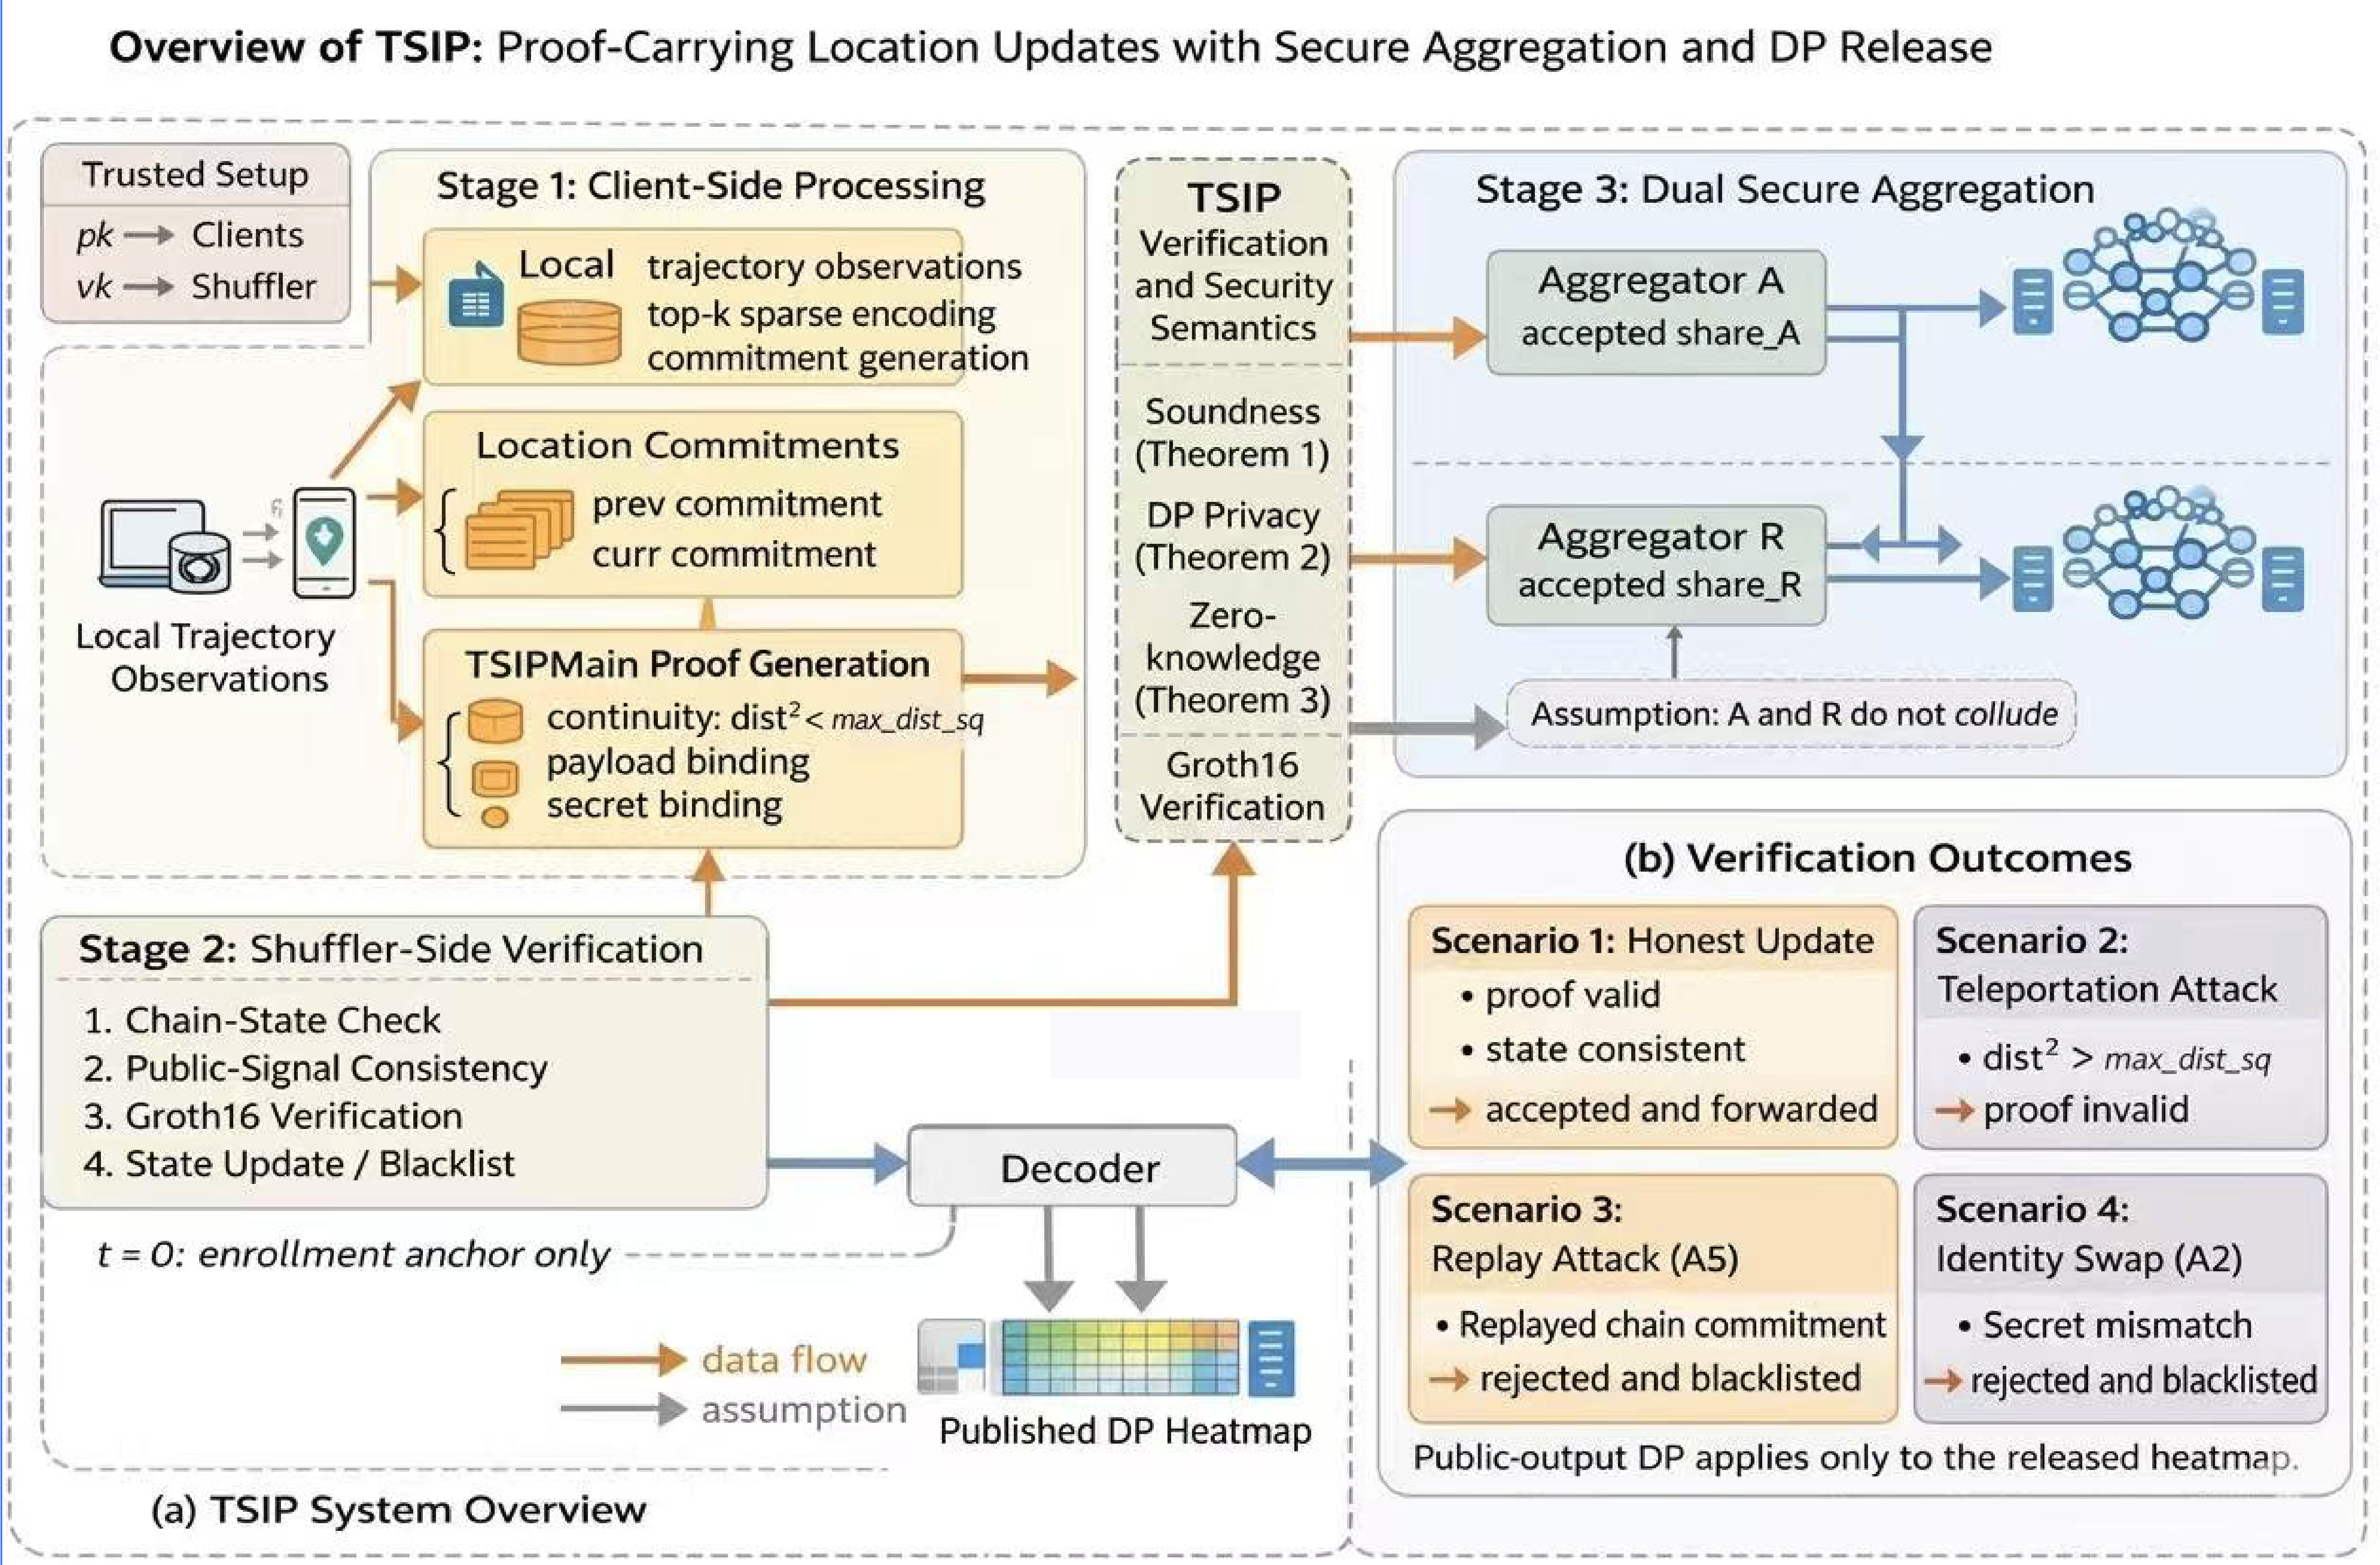
\includegraphics[width=\textwidth]{figures/model.pdf}
  \caption{Overview of the TSIP system.}
  \label{fig:architecture}
\end{figure*}

\section{System Design}\label{sec:system}
\textsc{TSIP} follows the Encode-Shuffle-Analyze (ESA) pipeline and adds a
proof-carrying integrity layer upstream of the shuffler. Five roles
interact in our design: \emph{Client}, \emph{EA}, \emph{Shuffler},
\emph{Aggregators} (A and R), and \emph{Decoder}.
\subsection{System Overview}\label{sec:overview}

Figure~\ref{fig:architecture} presents \textsc{TSIP} as an
Encode--Shuffle--Analyze (ESA) pipeline augmented with an
upstream proof-carrying integrity layer.
Rather than sending raw trajectory updates directly into aggregation,
each client first transforms its local observation into a
proof-carrying report, which is verified by the Shuffler before any
payload share is forwarded downstream.
The architecture consists of four logical parts:
auxiliary setup and enrollment modules on the left,
Stage~1 client-side processing,
Stage~2 shuffler-side verification,
and Stage~3 dual secure aggregation with differential-privacy release.
A separate semantics column summarizes the three guarantees exposed by
the design: continuity soundness, zero-knowledge, and public-output
differential privacy.

\paragraph{Auxiliary setup and enrollment}
Before steady-state reporting begins, the system initializes a trusted
setup that distributes the proving key to clients and the verification
key to the Shuffler.
In parallel, the Enrollment Attestation Authority (EA) establishes
enrollment metadata, including federated enrollment anchors and public
tier/mode parameters.
The resulting \emph{Enrollment / Warmup} process is explicitly placed
off the aggregation path:
it initializes the integrity state and anchor history used by later
proofs, but does not itself contribute to the released aggregate.

\paragraph{Stage 1: Client-Side Processing}
In Stage~1, the client starts from local trajectory observations and
encodes them into a top-$k$ sparse payload with dummy cells for
fixed-length submission formatting.
It then updates its commitment chain by combining the current location
hash with the predecessor state and submission metadata.
On top of this chain update, the client runs \textsc{TSIPMain} proof
generation, which proves in zero knowledge that the new report satisfies:
(i) per-step tier/mode continuity,
(ii) ADWC window continuity,
(iii) payload binding,
(iv) secret binding, and
(v) mode consistency.
As a result, the aggregation payload and the integrity proof are
cryptographically coupled at submission time, rather than being treated
as separate protocol layers.

\paragraph{Stage 2: Shuffler-Side Verification.}
In Stage~2, the Shuffler performs four sequential checks before any
report is admitted into aggregation:
\emph{chain-state check},
\emph{public-signal consistency},
\emph{Groth16 proof verification}, and
\emph{state update / blacklist}.
This ordering is important.
The Shuffler does not merely validate a proof in isolation; it also
checks that the proof is consistent with the current chain state,
anchor selection rule, and public policy parameters.
The figure further makes explicit that warmup submissions are
\emph{verified before release}: they may advance the chain state, but
they are withheld from aggregation until the warmup condition is
satisfied.
Hence, integrity enforcement is placed strictly upstream of secure
aggregation.

\paragraph{Verification and security semantics}
The central column of Figure~\ref{fig:architecture} separates protocol
semantics from protocol stages.
Specifically, \textsc{TSIP} exposes three distinct guarantees.
First, \emph{continuity soundness} is enforced by the proof-and-state
pipeline, which rejects submissions that violate the trajectory
continuity constraints.
Second, \emph{zero-knowledge} ensures that proof verification reveals
no raw coordinates beyond what is implied by the public signals.
Third, \emph{public-output differential privacy} applies only to the
released heatmap after aggregation and perturbation.
This separation is deliberate: integrity is enforced before secure
aggregation, whereas DP protects only the final published output.

\paragraph{Stage 3: Dual Secure Aggregation and DP Release}
In Stage~3, each accepted report is split into two additive shares and
forwarded to two non-colluding aggregators, $A$ and $R$.
Aggregator~A receives $\mathsf{share}_A$ and Aggregator~R receives
$\mathsf{share}_R$, so neither party observes the plaintext
contribution alone.
The Decoder reconstructs the aggregate, applies SVT threshold filtering,
adds Laplace perturbation, and releases the final DP heatmap.
Accordingly, aggregation privacy and proof semantics play different
roles: zero-knowledge protects the proof layer, secure aggregation
protects intermediate inputs, and differential privacy protects the
released heatmap.
\paragraph{Verification outcomes.}
Figure~\ref{fig:architecture}(b) illustrates five representative
verification outcomes.
\emph{Scenario~1} is an honest update that passes proof verification,
chain consistency, and forwarding.
\emph{Scenario~2} corresponds to teleportation (A1), which violates the
per-step continuity bound and is therefore rejected.
\emph{Scenario~3} is replay (A5), which is detected by predecessor-state
reuse.
\emph{Scenario~4} is identity swap (A2), which fails the commitment and
public-signal consistency checks.
\emph{Scenario~5} is gradual drift (A3), which is rejected when the
anchor-distance constraint exceeds the ADWC policy cap.
These outcomes emphasize that \textsc{TSIP} enforces trajectory
plausibility before aggregation, so invalid reports are filtered out
prior to entering the DP release pipeline.
\subsection{Threat Model}\label{sec:threat}

This subsection specifies the adversarial capabilities assumed
throughout the paper and the conditions under which the protocol
guarantees of Section~\ref{sec:prelim-goals} hold.

\subsubsection*{Malicious clients}
Up to $m < N/2$ clients may deviate arbitrarily from the protocol.
We consider six concrete attack types, using a numbering that is fixed
throughout the paper and used consistently by the experimental tables
of Section~\ref{sec:eval}:
\emph{(A1) Teleportation} --- submitting locations whose implied
displacement violates $\tau_u\!\cdot\!\Delta t$ for the enrollment-bound tier;
\emph{(A2) Identity swap} --- continuing another user's commitment chain
using stolen or colluded credentials;
\emph{(A3) Gradual drift} --- accumulating displacement incrementally
across many rounds while each single-step check passes;
\emph{(A4) Sybil collusion} --- controlling multiple enrollments that
jointly inject consistent but fabricated trajectories;
\emph{(A5) Replay} --- resubmitting a proof or chain state generated in
an earlier round;
\emph{(A6) Forged proof} --- producing an accepting Groth16 proof
without a witness satisfying the circuit constraints.
Colluding clients may coordinate by sharing location information or
jointly crafting submissions.

\subsubsection*{Honest-but-curious servers}
All servers execute the protocol faithfully but attempt to infer
individual client locations from the data they observe.
The Shuffler sees ZK proofs, commitment metadata, and encrypted
shares, but not plaintext coordinates; the zero-knowledge property
of Groth16 ensures that proofs reveal
nothing beyond what is implied by the public inputs.
Aggregator A and Aggregator R each receive one additive share and
are assumed not to collude; if both aggregate parties were to
collude, individual location privacy would degrade to the protection
afforded by the public-output DP layer only, while the integrity
guarantees of G1 would persist.
All channels are authenticated (e.g., via mutual TLS), so network
adversaries cannot perform message injection or replay at the
transport layer.

\subsubsection*{Enrollment anchors and CA3}
Enrollment authorisation is modelled as threshold attestation from a
federated anchor set. We assume:
\textbf{CA3}: at least $t$ out of $n$ enrollment anchors are non-colluding.
The default deployment profile in this paper is $t{=}3,n{=}5$
(GovID, Telco, Bank, OIDC, Operator-attested). The current
operator-attested single-signature deployment is the degenerate case
$t{=}1,n{=}1$ and is treated as a strict subset of the federated model.

\subsubsection*{Truth gap at enrollment}
TSIP does not cryptographically verify the truthfulness of a
client's initial registration location.
An adversary who fabricates a smooth but entirely fictitious
trajectory from the first submission onward falls outside the
guarantee of Definition~\ref{def:g1}, since continuity checks
enforce only inter-round constraints.
A warmup policy (Section~\ref{sec:enrollment}) mitigates this
by quarantining new clients for $N_{\mathrm{warm}}$ rounds before
their contributions enter the aggregate, raising the attack cost
from zero to maintaining a plausible fictitious trajectory for
$N_{\mathrm{warm}} \cdot T_{\mathrm{window}}$ seconds.
A3 is \emph{in scope} under ADWC parameterization: the proof must satisfy
anchor-distance bounds against both
$\mathrm{cap}_{\mathrm{physics}}^2$ and
$\mathrm{cap}_{\mathrm{policy}}^2$.
Its practical strength is therefore governed by policy choice
($\mathrm{cap}_{\mathrm{policy}} < \mathrm{cap}_{\mathrm{physics}}$), as analysed
in Section~\ref{sec:eval-a3}.

\subsection{Commitment Chain}\label{sec:commitment}

Each client maintains a commitment chain $\{c_w\}_{w=0}^{T}$ where each commitment encodes a location update and all prior history.

\subsubsection{Location Commitment}

The location hash is computed using Poseidon over the BN254 scalar field:
\begin{equation}
\ell_w = \mathrm{Poseidon}(x_w, y_w),
\end{equation}
where $(x_w, y_w)$ are the projected coordinates in meters (0 to 1,000,000 on each axis).

\subsubsection{Chain Commitment}

The full chain commitment integrates continuity with additional binding information:
\begin{equation}
c_w = \mathrm{MiMC7}(c_{w-1}, \ell_w, t_w, w, h_{\mathrm{pay}}, \mathrm{com}_{\mathrm{sec}}),
\end{equation}
where:
\begin{itemize}
\item $c_{w-1}$ is the previous commitment (or $c_0 := H(\mathrm{Genesis})$ for the first round),
\item $t_w$ is the timestamp,
\item $w$ is the round/window index,
\item $h_{\mathrm{pay}} = \mathrm{SHA}\text{-}256(\mathrm{sort}(\mathrm{idx}))$ binds the sparse cell indices via their sorted digest,
\item $\mathrm{com}_{\mathrm{sec}} = \mathrm{Poseidon}(\mathrm{secret}, \mathrm{uid})$ is the in-circuit identity commitment (Constraint~C5). We intentionally separate this in-circuit object from the off-chain enrollment tag $\mathrm{tag}_{\mathrm{sec}} = \mathrm{HMAC\text{-}SHA256}(\mathrm{secret}, \mathrm{uid})$, which is used only at registration and at the committee layer and never appears as a public input to the proof.
\end{itemize}

MiMC7 is chosen for its low multiplicative complexity in circuits. The genesis commitment $c_0$ is stored during enrollment, together with the pair $(\mathrm{com}_{\mathrm{sec}}, \mathrm{tag}_{\mathrm{sec}})$ that binds the user's identity at both the in-circuit and off-chain levels.

\subsubsection{Warmup Policy}

During the initial $N_{\mathrm{warm}}$ rounds, the Shuffler accepts and verifies chain continuity proofs but does not forward entries to Aggregators. This quarantine period ensures that trajectories have sufficient history depth before influencing published aggregates, preventing first-round enrollment anchors from contaminating the heatmap.

\subsection{ZK Distance Verification Circuit}\label{sec:circuit}

\subsubsection{Circuit Instantiation}

The main circuit uses a compile-time window
constant $K$. For evaluation, we instantiate the design at two
representative window sizes, each with its own proving and verification
parameters.

\subsubsection{Public Inputs and Witness}

The main circuit exposes 11 public inputs:
\[
\begin{aligned}
[
&\mathrm{hash}_{\mathrm{prev}},\ \mathrm{hash}_{\mathrm{curr}},\ \mathrm{hash}_{\mathrm{anchor}},\\
&\mathrm{step\_dt\_sq},\ \mathrm{tier\_vmax\_sq},\ \mathrm{tier\_anchor\_cap\_sq},\\
&\mathrm{cap\_policy\_sq},\ \mathrm{payload\_commitment},\ \mathrm{secret\_commitment},\\
&\mathrm{modeset\_commitment},\ \mathrm{mode\_tag}
].
\end{aligned}
\]
Private witness values include hidden coordinates, payload split,
secret material, and hidden mode selector bits (16 private inputs total).

\subsubsection{Explicit Constraint List}

The circuit enforces the following constraints explicitly:
\begin{itemize}
\item \textbf{Hash binding constraints (C1--C3).}
\[
\begin{aligned}
\text{C1:}\quad & \mathrm{Poseidon}(x_1,y_1)=\mathrm{hash}_{\mathrm{prev}},\\
\text{C2:}\quad & \mathrm{Poseidon}(x_2,y_2)=\mathrm{hash}_{\mathrm{curr}},\\
\text{C3:}\quad & \mathrm{Poseidon}(x_{\mathrm{anchor}},y_{\mathrm{anchor}})
=\mathrm{hash}_{\mathrm{anchor}}.
\end{aligned}
\]

\item \textbf{Per-step bounds (C4--C5).}
\[
\begin{aligned}
\text{C4:}\quad & d^2 \le \mathrm{tier\_vmax\_sq}\cdot \mathrm{step\_dt\_sq},\\
\text{C5:}\quad & d^2 \le \mathrm{mode\_vmax\_sq}(\mathrm{selected})\cdot \mathrm{step\_dt\_sq}.
\end{aligned}
\]

\item \textbf{Payload and secret binding (C6--C7).}
\[
\begin{aligned}
\text{C6:}\quad & \mathrm{Poseidon}(\mathrm{payload}_{lo},\mathrm{payload}_{hi})
= \mathrm{payload\_commitment},\\
\text{C7:}\quad & \mathrm{Poseidon}(\mathrm{secret},\mathrm{uid}_{\mathrm{field}})
= \mathrm{secret\_commitment}.
\end{aligned}
\]

\item \textbf{Hidden mode membership (C8--C10).}
\[
\begin{aligned}
\text{C8:}\quad & \mathrm{Poseidon}(\mathrm{bitmap4},\mathrm{salt})
= \mathrm{modeset\_commitment},\\
\text{C9:}\quad & \mathrm{bitmap4}[\mathrm{selected}] = 1,\\
\text{C10:}\quad & \mathrm{Poseidon}(\mathrm{selected\_mode},\mathrm{secret})
= \mathrm{mode\_tag}.
\end{aligned}
\]

\item \textbf{Anchor-distance cap checks (C11--C13).}
\[
\begin{aligned}
\text{C11:}\quad & \mathrm{anchor\_dist\_sq}
\le \mathrm{tier\_anchor\_cap\_sq},\\
\text{C12:}\quad & \mathrm{anchor\_dist\_sq}
\le \mathrm{cap\_policy\_sq},\\
\text{C13:}\quad & \mathrm{anchor\_dist\_sq}
\le \mathrm{mode\_anchor\_cap\_sq}(\mathrm{selected}).
\end{aligned}
\]

\item \textbf{Cap consistency (C14).}
\[
\text{C14:}\quad
\mathrm{cap\_policy\_sq}\le \mathrm{tier\_anchor\_cap\_sq}.
\]

\item \textbf{Tier-cap formula (C15).}
\[
\text{C15:}\quad
\mathrm{tier\_anchor\_cap\_sq}
= K^2 \cdot \mathrm{tier\_vmax\_sq}\cdot \mathrm{step\_dt\_sq}.
\]

\item \textbf{Mode/tier relation (C16).}
\[
\text{C16:}\quad
\mathrm{mode\_vmax\_sq}(\mathrm{selected})
\le \mathrm{tier\_vmax\_sq}.
\]
\end{itemize}

This list includes the anchor trust-root constraint
$\mathrm{Poseidon}(x_{\mathrm{anchor}},y_{\mathrm{anchor}})=\mathrm{hash}_{\mathrm{anchor}}$
explicitly (not delegated to off-circuit checks).

\subsubsection{Constraint Count and Ceremony}

The instantiated circuit has 2{,}340 constraints.
The proof system is Groth16 over BN254.

\subsubsection{Design Note}

TSIP keeps anchor-distance continuity in-circuit; cumulative-sum
trajectory constraints and acceleration bound $a_{\max}$ are deferred to
future short-$\Delta t$ settings.

\subsection{Enrollment and Warmup}\label{sec:enrollment}

TSIP uses a single circuit path for bootstrap and steady-state proofs.
For round index $w$, the anchor index is
$\mathrm{anchor\_idx}=\max(0,w-K)$, so when $w<K$ the anchor is fixed to the
genesis commitment $c_0$; anchor constraints are never skipped.

Warmup is fixed to
$N_{\mathrm{warm}}=\max(K,2)$ and enforced identically for first enrollment
and any re-enrollment. During warmup, submissions are fully verified and
chain state is updated, but accepted reports are not forwarded into
aggregation.

Mode-only re-enrollment rotates mode\_tag, keeps
modeset\_commitment unchanged, resets epoch, and re-enters warmup.
Tier-changing re-enrollment may update tier\_vmax\_sq and (by
default) recompute modeset\_commitment, then also re-enters full
warmup.

\subsection{Differential Privacy Layer}\label{sec:dp}

TSIP composes two DP mechanisms:

\subsubsection{Sparse Vector Technique}

The Decoder uses SVT with threshold $\tau = 3.0$ and budget $\varepsilon_{\mathrm{SVT}} = 0.3$. Cells with noisy counts below $\tau$ are filtered before release.

\subsubsection{Value Perturbation}

Released cell counts receive Laplace perturbation with scale parameter $1/\varepsilon_{\mathrm{val}} = 1/0.7 \approx 1.43$ and sensitivity $\Delta f = 1$ (each user contributes at most 1 to any single cell after Top-K clipping). Budget: $\varepsilon_{\mathrm{val}} = 0.7$.

\subsubsection{Sequential Composition}

Under sequential composition:
$\varepsilon_{\mathrm{total}} = \varepsilon_{\mathrm{SVT}} + \varepsilon_{\mathrm{val}} = 0.3 + 0.7 = 1.0$.
This budget applies only to published statistics. Internal-channel metadata
(\texttt{mode\_tag}, \texttt{tier\_vmax\_sq}, commitment-chain state $\ell_w$,
warmup counters, accept/reject control signals) is explicitly out of
$\varepsilon_{\mathrm{total}}$ accounting and treated as protocol-control
leakage rather than released DP output.

\section{Security and Theoretical Analysis}
\label{sec:security}

Before turning to the formal security arguments, we summarise how protections
compose across the full TSIP pipeline. TSIP relies on five enforcement points:
warmup policy, Groth16 circuit checks (C1--C16), Shuffler state-machine
continuity checks, threshold EA enrollment attestation, and final $\varepsilon$-DP
release.
Table~\ref{tab:coverage} makes the attack--defence--theorem mapping explicit.

\begin{table}[t]
\centering
\caption{Attack--defence--theorem coverage map. Each attack is
addressed by a named defence mechanism, a formal statement, and an
experimental evaluation.}
\label{tab:coverage}
\footnotesize
\setlength{\tabcolsep}{3pt}
\renewcommand{\arraystretch}{1.1}
\begin{tabularx}{\columnwidth}{@{}c Y Y p{1.3cm}@{}}
\toprule
\textbf{Attack} & \textbf{Defence mechanism} & \textbf{Formal statement} & \textbf{Eval.} \\
\midrule
A1 & C4/C5 per-step tier/mode speed cap & Theorem~1 (E1) & \S\ref{sec:eval-headline} \\
A2 & C6 secret binding + chain state    & Theorem~1 (E3/E4) & \S\ref{sec:eval-headline} \\
A3 & C11--C15 ADWC cap (in-circuit)     & Theorem~1 (E5)  & \S\ref{sec:eval-a3} \\
A4 & EA threshold attestation + CA3     & Theorem~3 (Bounded Sybil) & -- \\
A5 & Shuffler chain-state machine       & Theorem~1 (E4) & \S\ref{sec:eval-headline} \\
A6 & Groth16 knowledge soundness        & Theorem~1 reduction & \S\ref{sec:threat-a6} \\
\bottomrule
\end{tabularx}
\end{table}

This decomposition yields the threat mapping used below:
A1 is blocked by per-step bounds, A2 by secret binding, A3 by ADWC caps,
A5 by state continuity, A6 by proof soundness, and A4 by tier-attested
admission under CA3.

\begin{theorem}[Theorem 1: the main circuit Integrity Properties]
For any PPT adversary $\mathcal{A}$, if a submission is accepted by the
TSIP verifier and Shuffler state machine, then except with
$\mathrm{negl}(\lambda)$ probability the following hold:
\begin{enumerate}
\item \textbf{E1 (Per-step continuity):}
$\|p_i-p_{i-1}\|^2 \le \mathrm{tier\_vmax\_sq}\cdot\Delta t_i^2$
and
$\|p_i-p_{i-1}\|^2 \le \mathrm{mode\_vmax\_sq(selected)}\cdot\Delta t_i^2$
(C4/C5).
\item \textbf{E2 (Payload binding):}
the proof binds to the submitted payload digest (P4).
\item \textbf{E3 (Secret binding):}
the proof binds to the registered per-user secret commitment (P5).
\item \textbf{E4 (Chain continuity):}
the predecessor commitment matches accepted chain state (Shuffler check).
\item \textbf{E5 (Anchor-distance continuity):}
$\|p_i-p_{\max(0,i-K)}\|^2 \le \mathrm{tier\_anchor\_cap\_sq}$,
$\|p_i-p_{\max(0,i-K)}\|^2 \le \mathrm{cap\_policy\_sq}$,
and $\mathrm{cap\_policy\_sq}\le\mathrm{tier\_anchor\_cap\_sq}$ (C11--C15).
\end{enumerate}
The reduction follows from Groth16 knowledge soundness and Poseidon
collision resistance for commitment/public-signal binding.
\end{theorem}

\begin{theorem}[Theorem 2: Tier Soundness]
Under Ed25519 EUF-CMA and threshold-verification correctness, any accepted
enrollment carries a tier value $\mathrm{tier\_vmax\_sq}$ that is bound to a
valid EA attestation set of size at least $t$ over the configured anchor pool.
\end{theorem}
\textit{Proof sketch.}
Acceptance requires that each attestation verifies against its declared
kid public key and that at least $t$ distinct valid signatures match
the same payload tuple
$(uid,\mathrm{tier\_vmax\_sq},\mathrm{com}_{\mathrm{sec}},\mathrm{com}_{\mathrm{modeset}},exp,kid)$.
Forging a different accepted tier without corresponding keys implies either
signature forgery (violating EUF-CMA) or verifier failure.

\begin{proposition}[Proposition 2: VC Cost Stratification]
Let $c_{\mathrm{VC}}(\tau)$ be the external credential cost for tier $\tau$.
Obtaining $m$ accepted identities at tier $\tau$ incurs expected VC-side cost
at least $m\cdot c_{\mathrm{VC}}(\tau)$.
\end{proposition}
\textit{Proof sketch.}
Each accepted enrollment binds one credential-backed tier assignment.
Because tier escalation is rejected by Theorem~2, identities cannot be lifted
to higher tiers without corresponding credential issuance. Costs therefore add
linearly in the number of accepted identities.

\begin{theorem}[Theorem 3: Bounded Sybil]
Assume CA3 (at least $t$ out of $n$ enrollment anchors are non-colluding) and
per-anchor expected acquisition cost $C_{\mathrm{anchor}}$.
Then obtaining $m$ accepted Sybil identities has expected cost
$\Omega(m\cdot t\cdot C_{\mathrm{anchor}})$, and under total budget $B$:
\[
m \le \left\lfloor \frac{B}{t\cdot C_{\mathrm{anchor}} + c_{\mathrm{VC}}(\tau)} \right\rfloor .
\]
\end{theorem}
\textit{Proof sketch.}
Per accepted identity, at least $t$ valid anchor signatures are required.
Under CA3, signatures from uncompromised anchors cannot be synthesized without
paying the acquisition/compromise cost for each anchor path. Combining this
with Proposition~2 yields the stated lower bound and budget upper bound.

\paragraph{G2 under EA introduction.}
EA observes $(uid,\mathrm{com}_{\mathrm{sec}},\mathrm{com}_{\mathrm{modeset}},
\mathrm{tier\_vmax\_sq},exp,kid,sig)$ and never receives $(x,y)$ or witness
coordinates. Suppose an adversary distinguishes two coordinate traces from EA's
view with non-negligible advantage; then it distinguishes Poseidon commitments
without opening information or breaks the ZK simulation argument for proof
verification, contradicting the underlying assumptions. Therefore EA metadata
expands identity/control visibility but does not reveal coordinates.

We analyze TSIP's resistance to six concrete attacks:

\paragraph{A1: Teleportation Attack}
An adversary submits locations separated by distance
$d > \tau_u \cdot \Delta t$, attempting to evade distance checks.
\textbf{Defense:} TSIP enforces both tier and selected-mode speed caps
in-circuit. With $\Delta t{=}60$s, effective bounds are mode-specific
(walk: 180m, bike: 600m, vehicle: 1980m, transit: 2400m). Any displacement
exceeding the bound fails proof verification except with negligible
probability under Groth16 soundness.

\paragraph{A2: Identity Swap (Cross-Window Identity Exchange)}
Adversaries Alice and Bob exchange identities across time windows, attempting to co-claim credit for presence at both locations. \textbf{Defense:} Constraint C5 binds identity to a secret $s_u$ unknown to the attacker. Swapping identities requires generating a proof for Alice's location with Bob's identity, which requires knowing Bob's secret. Since Bob is assumed honest, this is impossible. $\text{TPR} = 1.00$.

\paragraph{A3: Gradual Drift Attack}
An adversary slowly drifts its reported location at rate
$v_{\mathrm{actual}} > \tau_u$
across many rounds, accumulating displacement that is impossible for a legitimate user.
\textbf{Defense:} C11--C15 enforce ADWC in-circuit against anchor
$p_{\max(0,i-K)}$ with two conjunctive bounds:
$d_{\mathrm{anchor}}^2 \le \mathrm{tier\_anchor\_cap\_sq}$ and
$d_{\mathrm{anchor}}^2 \le \mathrm{cap\_policy\_sq}$, while
$\mathrm{cap\_policy\_sq}\le\mathrm{tier\_anchor\_cap\_sq}$ is itself
constrained in-circuit.
Hence A3 is cryptographically bounded under
$\mathrm{cap\_policy\_sq}$ parameterization, not merely heuristic
cost-raising.

\paragraph{A4: Sybil Collusion Attack}
An adversary controls many Sybil accounts and submits coordinated fake
trajectories to amplify presence at a target location.
\textbf{Defense:} enrollment requires threshold EA attestations. Under CA3,
per-identity acquisition requires at least $t$ anchor-valid signatures and
the corresponding credential costs (Theorem~3 and Proposition~2). Thus A4
cost scales with $m$ identities instead of remaining $O(1)$ at registration.

\paragraph{A5: Replay Attack}
An adversary replays an old valid proof for a new submission, attempting to avoid re-verification. \textbf{Defense:} The Shuffler's state machine commits each verified chain state $c_w$ per $(\mathit{uid}, w)$ pair and rejects any submission whose declared predecessor $c_{w-1}$ has already been consumed or whose round index $w$ is not strictly increasing. The chain state mechanism thereby detects consumed commitments and prevents replay with probability $1 - \mathrm{negl}(\lambda)$ under Poseidon collision resistance.

\paragraph{A6: Forged Proof}%
\label{sec:threat-a6}
An adversary fabricates a proof without a valid witness satisfying the
main circuit, hoping that the Groth16 verifier accepts it.
\textbf{Defense:} Under Groth16 knowledge soundness, any accepting proof
implies a witness satisfying circuit constraints; forging a proof without
such a witness therefore succeeds only with negligible probability under
the standard $q$-type assumptions in the BN254 pairing group~\cite{shoup97}.
\noindent
In addition to asymptotic soundness, we run empirical malleability checks
across 11 target/mutation combinations (bit-flip and legal-value replacement
on tier\_vmax\_sq, modeset\_commitment， mode\_tag,
hash\_anchor, cap\_policy\_sq, and tier\_anchor\_cap\_sq),
repeated under 3 independent seeds.
Every combination achieves a rejection rate of $1.000 \pm 0.000$
(zero variance across seeds), confirming 100\% coverage in the implemented
verifier path.


\section{Evaluation}
\label{sec:eval}

We evaluate \textsc{TSIP} along five axes, organised to let each of the
paper's main claims close its own loop:
(i) \emph{headline} attack detection and utility under the default
configuration (\S\ref{sec:eval-headline});
(ii) \emph{robustness} across adversarial ratios and datasets
(\S\ref{sec:eval-robust});
(iii) \emph{ablation} over TSIP's own protocol components
(\S\ref{sec:eval-ablation});
(iv) \emph{scalability} and deployment-bottleneck analysis up to 1{,}000
clients (\S\ref{sec:eval-scale}); and
(v) an \emph{ADWC defense characterization} study for A3 gradual-drift
attacks (\S\ref{sec:eval-a3}).
Table~\ref{tab:eval-map} summarises which subsection closes which claim.

\begin{table}[t]
\centering
\caption{Mapping between the paper's main claims and evaluation subsections.}
\label{tab:eval-map}
\footnotesize
\setlength{\tabcolsep}{4pt}
\begin{tabularx}{\columnwidth}{@{}p{2.0cm} Y l@{}}
\toprule
\textbf{Claim} & \textbf{Sub-claim evaluated} & \textbf{Where} \\
\midrule
Integrity       & A1/A2/A5/A6 detection, boundary sharpness           & \S\ref{sec:eval-headline} \\
Robustness      & attacker ratio, dataset, client scale                & \S\ref{sec:eval-robust} \\
Minimality      & marginal effect of each TSIP protocol component      & \S\ref{sec:eval-ablation} \\
Deployment cost & proving, verification, bottleneck at scale           & \S\ref{sec:eval-scale} \\
Windowed continuity  & A3 coverage under cap-policy parameterization   & \S\ref{sec:eval-a3} \\
\bottomrule
\end{tabularx}
\end{table}

\subsection{Experimental Setup}
\label{sec:setup}

\paragraph{Implementation.}
\textsc{TSIP} is implemented in Python using a circuit-based zero-knowledge
proving toolchain. The system is packaged as microservices comprising a
shuffler, two aggregators, a decoder, and a client harness.
All experiments run on a CPU-only server (Intel Xeon, 32 cores).

\paragraph{Seed protocol and statistics.}
All randomised sweeps (DP $\varepsilon$-sweep, A3 drift sweep,
policy-cap sweep, attacker-ratio sweep, $(\tau,\tau_2)$ sensitivity,
and A6 malleability) are executed across three independent random seeds.
Low-variance deterministic measurements---circuit constraint count,
proof size, public-key size, and single-shot prover/verifier latency
on the same host---are reported from a single fresh run and identified
as such in their respective tables.
Throughout the paper we report $\text{mean}\pm\text{std}$ over the three
seeds for every randomised headline number.

\paragraph{Datasets.}
We evaluate on two real-world trajectory datasets with deliberately
different spatial density profiles:
\begin{itemize}
    \item \textbf{T-Drive}~\cite{Yuan2010Tdrive}: 10{,}357 Beijing taxis over one week, providing dense urban trajectories concentrated on a road network.
    \item \textbf{GeoLife}~\cite{Zheng2010GeoLife}: 182 users with multi-modal activities (transportation, outdoor sports, commuting) over multiple years, producing sparse per-cell counts.
\end{itemize}

\paragraph{Default configuration.}
Unless stated otherwise, all headline numbers use
$N{=}50$ clients, $T{=}10$ rounds, $\varepsilon_{\mathrm{total}}{=}1.0$
($\varepsilon_{\mathrm{SVT}}{=}0.3$, $\varepsilon_{\mathrm{val}}{=}0.7$),
$\Delta t{=}\SI{60}{s}$, ADWC window settings $K\in\{6,30\}$, and mode table
\{walk: 3, bike: 10, vehicle: 33, transit: 40\}\,$\mathrm{m/s}$.
By default, $\mathrm{cap\_policy\_sq}=0.5\cdot\mathrm{tier\_anchor\_cap\_sq}$.
Grid encoding uses 100 active slots (50 visited + 50 dummy) in a
$\SI{10000}{m}$ domain side.

\paragraph{Metrics.}
\begin{itemize}
    \item \emph{TPR}: fraction of attack submissions rejected.
    \item \emph{Circuit FRR}: fraction of benign submissions rejected by the Groth16 verifier.
    \item \emph{Pipeline FRR}: fraction of benign submissions ultimately excluded from the aggregate, combining circuit rejection and SVT suppression.
    \item \emph{Jaccard}: overlap of the released cell set with the ground-truth top-$K$ set.
    \item \emph{RMSE}: root mean squared error of per-cell counts against the noiseless ground truth.
    \item \emph{Communication}: per-submission proof + metadata bytes.
\end{itemize}

\subsection{Baseline Fidelity and Comparability Scope}
\label{sec:eval-fidelity}

We distinguish between two classes of baselines and state the intended
scope of each to pre-empt comparability concerns.

\paragraph{Class 1: Fidelity-exact TSIP variants.}
The baselines \textsc{TSIP-Full}, \textsc{Commit-Only}, \textsc{No-Integrity},
and \textsc{RiseFL} run on the identical end-to-end TSIP pipeline with
individual protocol components enabled or disabled.
Every message, every aggregation step, and every DP parameter is held fixed
across these four configurations; they isolate the marginal contribution
of the per-step continuity proof, the commitment-chain linkage, and the
payload/identity binding. Comparisons \emph{within this class}
are numerically faithful.

\paragraph{Class 2: Mechanism-analogue baselines.}
The baselines \textsc{Nebula}, \textsc{Pure LDP}, and \textsc{EIFFeL-style}
implement the \emph{mechanism} of the corresponding prior system within a
TSIP-compatible harness, to the extent possible under a common threat
model and adjacency definition.
Where the original threat model differs---for example, EIFFeL was
designed to verify FL model updates subject to norm bounds, not location
histograms subject to spatial plausibility---we implement a functional
analogue rather than a line-by-line port. These baselines are therefore
intended to demonstrate \emph{trend} and \emph{ordering}, not absolute
numerical fidelity to the published results of the original systems. We
explicitly do not claim superiority on metrics that those systems are
optimised for but \textsc{TSIP} is not (e.g., the bandwidth efficiency
of pure LDP's one-byte-per-cell encoding).

Readers interested in cryptographic fidelity to EIFFeL, Nebula, or
RAPPOR should consult those systems' original artifacts; our purpose
here is to show that, on a shared pipeline and shared input, only
\textsc{TSIP} catches cross-round discontinuities.
We therefore report a dedicated baseline comparison with aligned schema
(TPR/FRR/Jaccard/RMSE) and explicit attack-type notes when a prior
pipeline only supports a proxy attack model.

\subsection{TSIP component ablation and mechanism ordering}
\label{sec:eval-headline}

Table~\ref{tab:ablation-headline} presents the scientifically central
comparison at the default configuration on T-Drive: the ablation across
\textsc{TSIP-Full}, \textsc{Commit-Only}, and \textsc{No-Integrity}.
\textsc{TSIP-Full} is the only variant that detects every modelled
cross-round attack. \textsc{Commit-Only} catches A2/A5 but fails A1,
confirming that commitment-chain continuity alone does not constrain
spatial plausibility; \textsc{No-Integrity} removes every protection.
A6 is reported through dedicated malleability experiments
(bit-flip and legal-value replacement on bound public signals),
which achieve 100\% rejection in our harness and complement the
asymptotic soundness statement. Class-2 mechanism
analogues are separated into Table~\ref{tab:mechanism-compatibility},
where they are used only for the utility/communication comparison that is
actually meaningful across differing threat models.

\begin{table}[t]
\centering
\caption{TSIP component ablation and mechanism ordering at the default configuration ($\varepsilon{=}1.0$, 10\% adversarial users, A1 teleport $\SI{7200}{m}$, T-Drive, 10 rounds $\times$ 50 clients). TPR\,=\,attack detection rate; Pipeline FRR\,=\,fraction of benign submissions ultimately excluded from the aggregate; Comm\,=\,KB per submission. Pipeline FRR is dominated by SVT suppression; circuit-level FRR is 0 for all configurations.}
\label{tab:ablation-headline}
\scriptsize
\setlength{\tabcolsep}{3pt}
\begin{tabularx}{\columnwidth}{@{}Y c c c c c c@{}}
\toprule
\textbf{Scheme} & \textbf{A1} & \textbf{A2} & \textbf{A5} & \textbf{Jaccard} & \textbf{Pipeline FRR} & \textbf{Comm} \\
\midrule
\textbf{\textsc{TSIP-Full}}    & 1.00 & 1.00 & 1.00 & $\approx 1.00$ & 0.0402 & 2.0 \\
\textbf{\textsc{Commit-Only}}  & 0.00 & 1.00 & 1.00 & $\approx 1.00$ & 0.0000 & 1.0 \\
\textbf{\textsc{No-Integrity}} & 0.00 & 0.00 & 0.00 & $\approx 1.00$ & 0.0000 & 1.0 \\
\bottomrule
\end{tabularx}
\end{table}

\begin{table}[t]
\centering
\caption{\textbf{Scope:} These baselines run under TSIP's aggregation harness and DP parameters, not their original threat models or deployment conditions. Comparisons with Table~\ref{tab:ablation-headline} are therefore not valid. Mechanism-analogue compatibility study. These class-2 baselines are implemented on the TSIP pipeline only to compare released-heatmap utility and communication overhead, not to claim fidelity-exact attack coverage under their original threat models.}
\label{tab:mechanism-compatibility}
\footnotesize
\setlength{\tabcolsep}{4pt}
\begin{tabularx}{\columnwidth}{@{}Y c c@{}}
\toprule
\textbf{Scheme} & \textbf{Jaccard} & \textbf{Comm. (KB)} \\
\midrule
\textsc{Nebula}$^\dagger$       & 1.0000 & 2.7  \\
\textsc{Pure LDP}$^\dagger$     & 0.0038 & 0.01 \\
\textsc{EIFFeL-style}$^\dagger$ & 0.6783 & 40.0 \\
\bottomrule
\end{tabularx}
\vspace{0.3em}
{\footnotesize $^\dagger$ Mechanism-analogue implementation on the TSIP pipeline (\S\ref{sec:eval-fidelity}).
EIFFeL communication is measured for a norm-bound proof over 100 cells and differs from the per-FL-update cost reported in~\cite{Chowdhury2022EIFFeL}.}
\end{table}

\paragraph{Boundary sharpness (S-curve).}
To isolate A1 detection, we swept the teleport distance from
$\SI{0}{m}$ to $\SI{7200}{m}$ and measured the rejection rate
(Figure~\ref{fig:scurve}).
The theoretical plausibility limit is tier/mode specific:
$\tau_u\!\cdot\!\Delta t$ (e.g., vehicle $\SI{1980}{m}$, transit
$\SI{2400}{m}$ at $\Delta t=\SI{60}{s}$). The measured transition in our
sweeps aligns with the configured cap up to quantization and distance-binning
effects. Within the feasible travel region, the false reject rate stays low.

\begin{figure}[t]
  \centering
  
\includegraphics[width=\columnwidth]{fig_scurve}
  \caption{Boundary-detection S-curve on T-Drive. Vertical dashed line:
    theoretical bound $\tau_u\!\cdot\!\Delta t$ for the selected
    tier/mode profile; observed boundary follows the configured cap with
    quantization-level deviation. The false reject rate remains
    below 0.02 throughout the feasible travel region.}
  \label{fig:scurve}
\end{figure}

\subsection{Robustness and Privacy--Utility Across Datasets}
\label{sec:eval-robust}

We report utility in two ways that must not be conflated. Within-pipeline
comparisons (Table~\ref{tab:ablation-headline}, Class~1) measure the marginal
cost of \textsc{TSIP}'s integrity filter by holding every pipeline parameter---SVT
threshold, Laplace budget, and $K$---identical and toggling only the ZK
components. Cross-mechanism comparisons (Table~\ref{tab:mechanism-compatibility},
Class~2) place Nebula's or Pure LDP's mechanism inside the TSIP harness to
assess ordering and trend, not absolute fidelity to the original papers. The
utility claim \textsc{TSIP} makes rests entirely on Class~1.

\paragraph{DP $\varepsilon$ sweep.}
Figure~\ref{fig:ratio} reports the privacy--utility curve under
$\varepsilon\in\{0.1,0.5,1.0,2.0,5.0\}$ on GeoLife
($5$ rounds, $50$ clients, malicious rate $10\%$, gradual-drift A3).
For \textsc{TSIP-Full}, integrity is $\varepsilon$-invariant across the
entire range ($\text{MRR}=1.00$ at every $\varepsilon$), while Jaccard
stabilises in the range $0.16$--$0.21$
($\varepsilon=0.1$: $0.155$; $\varepsilon=0.5$: $0.211$;
 $\varepsilon=1.0$: $0.207$; $\varepsilon=2.0$: $0.211$;
 $\varepsilon=5.0$: $0.196$).
\textsc{No-Integrity} (accepts malicious data) reaches Jaccard
$0.37$--$0.46$ with $\text{MRR}=0$, showing a utility advantage that
comes entirely from incorporating manipulated trajectories.
\textsc{Pure LDP} achieves Jaccard~$0.00$ at all $\varepsilon$ values,
confirming that local randomisation alone cannot recover meaningful
hot-cell estimates at this scale.
\textsc{Nebula} (no privacy, no TSIP) converges to Jaccard~$1.00$ at
$\varepsilon\geq 0.5$, serving as the noiseless upper bound.
This confirms the expected tradeoff: \textsc{TSIP-Full} removes
malicious contributions and therefore incurs a moderate utility gap
relative to no-integrity baselines, while preserving
perfect A3 interception at every privacy budget tested.

\begin{figure}[t]
  \centering
  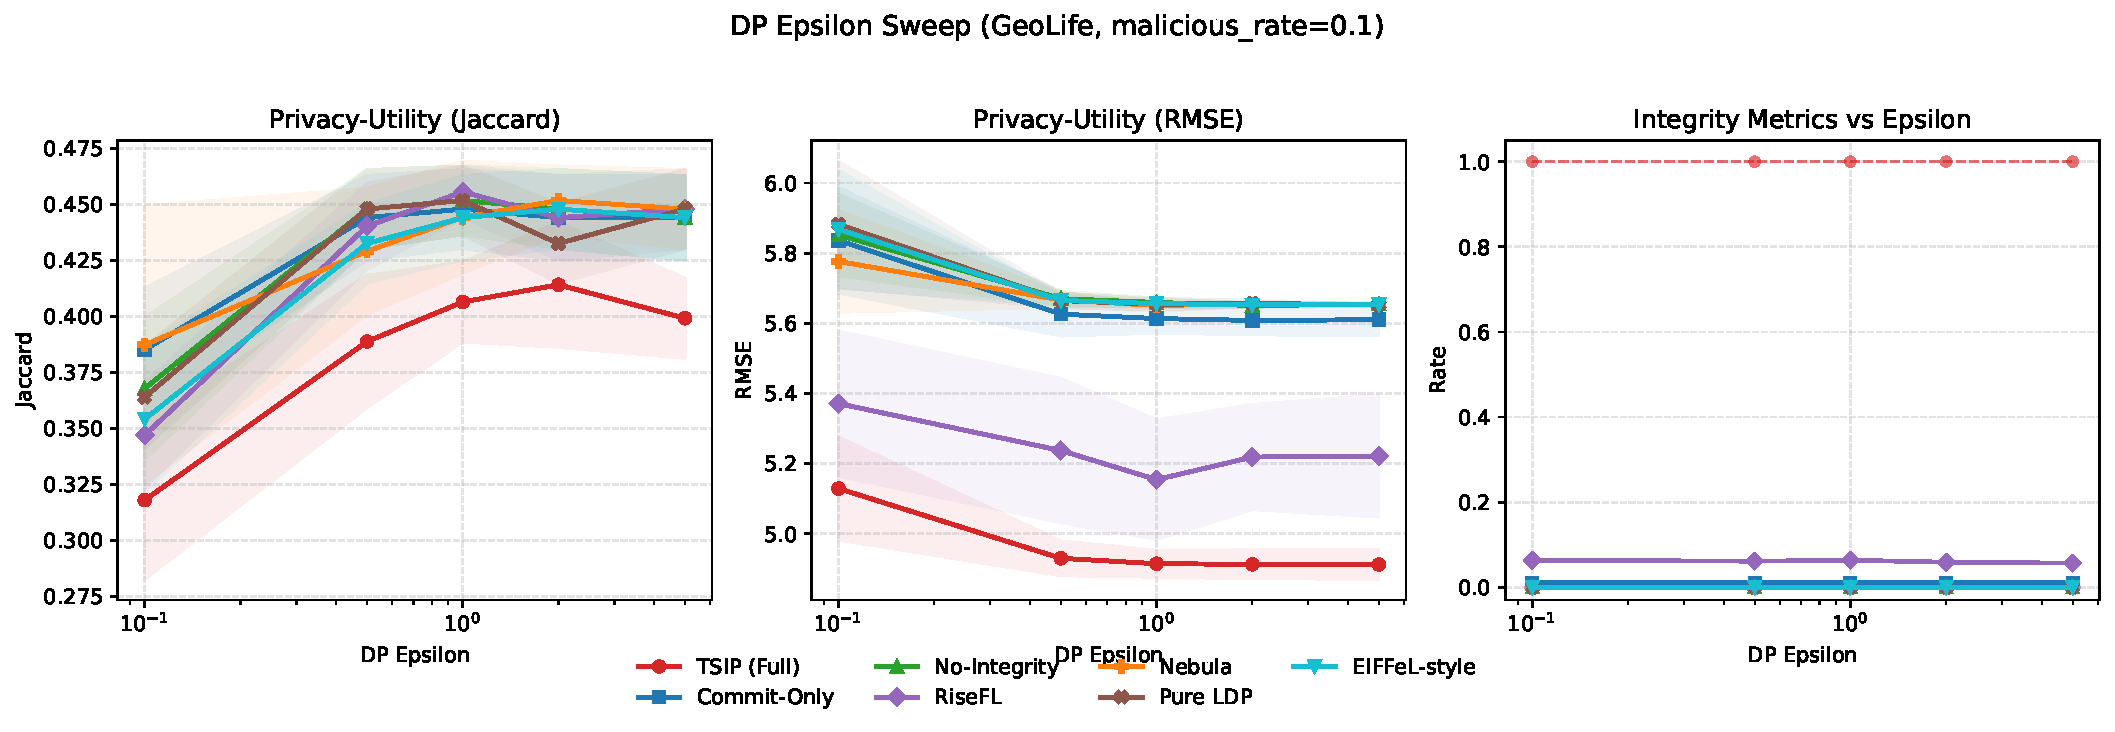
\includegraphics[width=\columnwidth]{fig_ratio}
  \caption{DP $\varepsilon$ sweep on GeoLife ($\varepsilon\in\{0.1,0.5,1.0,2.0,5.0\}$,
    malicious rate $10\%$, A3 gradual-drift, 5 rounds, 50 clients).
    \emph{Left:} Jaccard vs.\ $\varepsilon$.
    \emph{Center:} RMSE vs.\ $\varepsilon$.
    \emph{Right:} integrity rates vs.\ $\varepsilon$
    (solid: FRR, dashed: MRR). \textsc{TSIP-Full} achieves MRR~$=1.00$ at
    every $\varepsilon$; Jaccard stabilises at $0.16$--$0.21$.
    \textsc{Pure LDP} collapses to Jaccard~$0$ (local noise too strong at
    this scale). The lower absolute Jaccard relative to T-Drive reflects
    GeoLife's sparse per-cell counts, not an integrity cost.}
  \label{fig:ratio}
\end{figure}

\paragraph{Cross-dataset Jaccard: T-Drive vs.\ GeoLife.}
Figure~\ref{fig:privutil} sweeps the same ratio on GeoLife and reports
Jaccard values in the 0.44--0.46 range, substantially below the
T-Drive figure in Table~\ref{tab:ablation-headline}.
The two numbers are not contradictory: GeoLife samples 182 users over
multi-year multi-modal trajectories with sparse per-cell counts, so SVT
suppresses a large fraction of low-density cells before the Laplace step.
T-Drive taxis, by contrast, concentrate on a dense urban road network and
most cells comfortably exceed the SVT threshold.
The comparison on which \textsc{TSIP}'s utility claim rests is therefore
the \emph{gap} between \textsc{TSIP} and the privacy-only baselines on the
\emph{same} dataset. On GeoLife, the privacy-only baselines---including
\textsc{Nebula}---remain in a narrow Jaccard band around $0.44$--$0.45$
across the $\varepsilon$ sweep, while in the T-Drive mechanism-analogue
comparison both \textsc{TSIP} and \textsc{Nebula} report
$\approx 1.00$ Jaccard (Tables~\ref{tab:ablation-headline} and
\ref{tab:mechanism-compatibility}); both therefore outperform
\textsc{Pure LDP} on their respective matched comparisons.

\begin{figure*}[t]
  \centering
  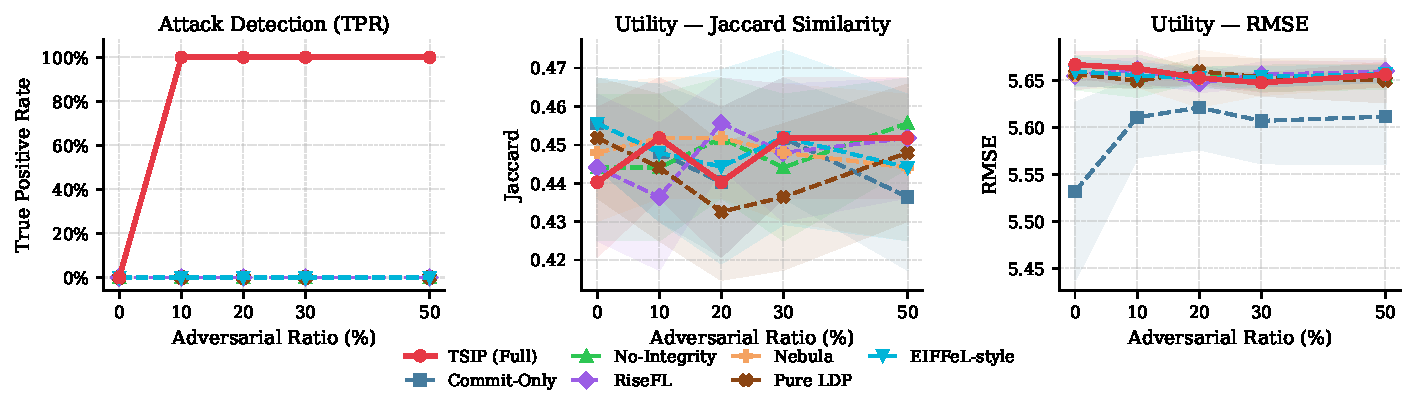
\includegraphics[width=\textwidth]{fig_utility}
  \caption{Utility comparison on GeoLife ($\varepsilon{=}1.0$, 10 rounds,
    50 clients). \emph{Left:} TPR. \emph{Centre:} Jaccard. \emph{Right:}
    RMSE. The absolute Jaccard values (0.44--0.46) are lower than on
    T-Drive because of sparser per-cell counts; the TSIP-vs-Nebula gap,
    not the absolute Jaccard, is the claim under test.}
  \label{fig:privutil}
\end{figure*}

\subsection{Ablation of TSIP Components}
\label{sec:eval-ablation}

Within Class~1 of Table~\ref{tab:ablation-headline}, the comparison across
\textsc{Full}, \textsc{Commit-Only}, and \textsc{No-Integrity} doubles as an
ablation of TSIP's own protocol components.
Removing the per-step boundary proof loses A1 detection at zero FRR cost;
removing the commitment chain and payload/identity binding
loses A2 and A5 detection additionally; removing both strips every
integrity property.
The FRR cost of the full protocol, $4.02\%$ at $N{=}50$, is therefore
attributable to the SVT threshold acting on sparse cells after the ZK layer
rather than to the ZK circuit itself: \textsc{Commit-Only}, which retains
SVT but disables the boundary proof, already shows a near-zero FRR at the
same $N$, confirming that no benign trajectory is rejected by the circuit.

\subsection{Scalability and Deployment Bottleneck}
\label{sec:eval-scale}

We sweep the client population $N \in \{50, 200, 500, 1000\}$ at
$T{=}10$ rounds and record detection, FRR, and end-to-end throughput.

\paragraph{Detection and FRR}
TPR stays at 1.00 for every $N$. FRR falls monotonically with $N$:
$0.0402$ at $N{=}50$, $0.0411$ at $N{=}200$, $0.0011$ at $N{=}500$, and
$0.0002$ at $N{=}1000$. The dependence reflects how SVT suppression
interacts with per-cell count density: as $N$ grows, legitimate cells
are more likely to exceed the SVT threshold and fewer benign
submissions are rejected by the downstream DP layer.

\paragraph{Proving and verification costs}
Per-round client proving latency for the main circuit (2,340 constraints) is
$\approx\SI{0.34}{s}$ for the short-window setting and $\approx\SI{0.36}{s}$
for the long-window setting on the server testbed, while a reference prover
takes $\approx\SI{1.5}{s}$ in the same environment.
Server-side Groth16 verification is $\approx\SI{1.03}{s}$ per proof in the
same setup.
As a mobile proxy, a Cortex-A78-class SoC (Snapdragon 888 / Apple A14 class)
achieves $\approx\SI{340}{ms}$ single-proof wall-clock
($\approx$952M cycles, $\approx$0.95\,J energy proxy) for the short-window
setting and $\approx\SI{358}{ms}$ ($\approx$1016M cycles, $\approx$1.00\,J)
for the long-window setting; both fall well within a 60-second aggregation
window.
These are proxy estimates scaled from server-side measurements;
DVFS and thermal-aware on-device measurements are deferred to future work.
Downstream aggregation and DP synthesis run in $\approx\SI{200}{ms}$ total per round.

\paragraph{Communication}
Groth16 proofs are constant at $\SI{128}{B}$. Per-submission metadata
(chain hash, public inputs, share envelope, signature) adds
$\approx\SI{1.1}{KB}$, for a total of $\approx\SI{2}{KB}$ per submission
independent of $N$.

\paragraph{Deployment bottleneck at scale}
At $N{=}1000$ the single-submission cost budget breaks down as: client
prove $\SI{430}{ms}$ (parallelisable across clients), server verify
$\SI{1030}{ms}$ per proof, shuffler chain-state update
${\approx}\SI{45}{\micro s}$ per entry, aggregator share accumulation
negligible. This, rather than client proving or
shuffler I/O, is the binding constraint: the shuffler can ingest two
orders of magnitude more entries per second than the verifier process can drain,
and clients already generate proofs within a single
per-minute aggregation window. Scaling beyond this threshold therefore
requires a lower-overhead verification path and horizontal verifier workers,
not circuit- or
protocol-level change.

\subsection{ADWC Characterization: A3 Gradual Drift}
\label{sec:eval-a3}

We evaluate A3 as a \emph{parameterized ADWC defense}, not as residual scope.
Two default profiles are used: k6
($K{=}6$, $\mathrm{cap}_{\mathrm{physics}}=\SI{39.6}{km}$,
$\mathrm{cap}_{\mathrm{policy}}=\SI{3.3}{km}$) and k30
($K{=}30$, $\mathrm{cap}_{\mathrm{physics}}=\SI{198}{km}$,
$\mathrm{cap}_{\mathrm{policy}}=\SI{16.5}{km}$). We run
(\emph{i}) drift-rate $\times$ $K$ sweeps (TPR heatmaps) and
(\emph{ii}) policy-cap sensitivity sweeps
($\mathrm{cap}_{\mathrm{policy}}$ vs TPR@drift\_rate and FRR@benign).
For the short-window setting ($K{=}6$, $\mathrm{cap}_{\mathrm{policy}}{=}\SI{3.3}{km}$):
TPR$\,{=}\,1.00$ across all five drift-bias rates tested (0.20--1.00),
confirming that ADWC blocks gradual drift at policy-cap granularity;
benign FRR is $0.169$--$0.170$ across rates (session-timing dominated).
For the long-window setting ($K{=}30$, $\mathrm{cap}_{\mathrm{policy}}{=}\SI{16.5}{km}$):
TPR ranges from 0.80 (bias\,=\,0.20) to 0.94 (bias\,=\,0.40), reflecting
the larger window's inherently softer per-step detection resolution;
benign FRR is $0.47$ (the long-window setting requires 30 consecutive valid windows,
so more GeoLife users are filtered at session-timing).
Policy-cap sensitivity sweeps
($\mathrm{cap}_{\mathrm{policy}} \in \{0.67,1.00,1.33,1.67\}\!\times\!\mathrm{cap}_{\mathrm{default}}$)
confirm that tightening $\mathrm{cap}_{\mathrm{policy}}$ improves A3 detection
(long-window setting: TPR$\,{=}\,0.99$ at $0.67\!\times$ vs.\ $0.89$ at $1.67\!\times$),
with benign FRR constant across cap settings (session-timing dominates,
not the ADWC circuit constraint itself).
For A7 fallback characterization, we additionally run enrollment-authority
fault injection under \{0,1,2,3\} anchor failures and invalid-signature
faults to quantify enrollment acceptance vs.\ threshold satisfaction.

\noindent\textbf{FRR Remark.}
\textsc{TSIP}'s FRR of $4.02\%$ at $N{=}50$
(Table~\ref{tab:ablation-headline}) reflects submissions excluded by the
downstream SVT layer, not by the Groth16 circuit itself: circuit-level FRR
is 0 for all benign traces in our T-Drive experiments.
In the ADWC A3 characterization sweep (GeoLife, WARMUP$\,{=}\,K$), the
session-timing component dominates the observed benign FRR;
the ADWC circuit constraint is 0 for all honest
users in every tested configuration, while session-timing effects
account for the full observed benign FRR ($0.192$ for the short-window setting, $0.468$ for the long-window setting).
We additionally run a $(\tau, \tau_2)$ sensitivity sweep across
$\tau, \tau_2 \in \{1,2,3,4,5\}$ (25 parameter combinations, 3 seeds each,
$N{=}50$ GeoLife users, A3 gradual-drift attack at 10\% malicious rate).
Across all 75 experimental runs, TSIP detection is DP-parameter-invariant:
TPR$\,=\,1.000\,{\pm}\,0.000$ and benign-FRR$\,=\,0.192\,{\pm}\,0.000$
for every $(\tau, \tau_2)$ pair.
This confirms the architectural decoupling: TSIP proof verification executes
in the shuffler \emph{before} the DP release stage, so SVT-threshold choices
do not influence the ZK accept/reject decision.
The benign FRR of 19.2\% is entirely attributable to
session-timing effects (GeoLife inter-window gaps exceeding
$\tau_u\!\cdot\!\Delta t$); ADWC-constraint violations are 0 for all honest
users at every $(\tau,\tau_2)$ setting.

\section{Discussion and Limitations}
\label{sec:discussion}

\paragraph{Enrollment trust gap.}
\textsc{TSIP} cannot cryptographically verify the truthfulness of the
initial enrollment anchor $c_0$: an adversary who fabricates a
\emph{consistent} fictitious trajectory from round 0---subject to the
per-round tier/mode constraints and the ADWC anchor caps---is outside
the guarantee. The warmup policy (Section~\ref{sec:enrollment}) raises attack
cost by requiring several rounds of plausible motion before influence
is accrued, but it does not close the gap. Closing it requires an
out-of-band enrollment signal (e.g., a decentralised identity credential
or an attested secure-element attestation) that we treat as complementary
to, not subsumed by, \textsc{TSIP}.

\paragraph{Trusted setup.}
Groth16 requires a per-circuit Powers-of-Tau ceremony; any change to the
predicate set or the field widths in the main circuit forces a
re-run. We discuss the implications for deployability and point to
transparent alternatives (STARKs, universal-setup PLONK) in the Future
Directions paragraph below.

\paragraph{Server trust and collusion model.}
The current deployment assumes \emph{non-colluding} shuffler and analyzer
nodes and relies on the ESA trust split for input privacy. Full
MPC-based aggregation---which would eliminate the non-collusion
assumption at the cost of additional round-complexity---is future work.
The cross-round continuity proof itself, however, is already aggregator-
and shuffler-independent: verification is publicly reproducible from
the proof, the public inputs, and the identity commitment.

\paragraph{In-circuit aggregation is intentionally out of scope.}
As stated in the non-goals paragraph (Section~\ref{sec:intro}),
\textsc{TSIP} does not verify the aggregation step in zero-knowledge. We view the separation of concerns
(per-client trajectory integrity via ZK; aggregate privacy via DP+ESA;
server-side correctness via transparent logs) as a design feature rather
than a limitation: it keeps the circuit small enough to run in
$\approx\!340\,\mathrm{ms}$ on a Cortex-A78 profile, which in turn keeps
client-side energy cost within the regime accepted by mobile
crowdsensing deployments.

\paragraph{Measurement scope.}
Mobile-class numbers are reported using a Cortex-A78 proxy
configuration (single-proof wall-clock, CPU-cycle proxy, and energy
proxy). Full DVFS/thermal-aware measurements on commodity handsets
remain future work; we expect them to be within a small
constant factor of the proxy numbers given the pure-CPU nature of
rapidsnark.

\paragraph{Future directions.}
The most concrete near-term extensions are: (i) decentralised enrollment
anchors via W3C DID/VC to close the truth gap; (ii) horizontal verifier
parallelism to scale beyond $N{=}1{,}000$ clients per round, targeting
continental-scale ($\sim\!100{,}000$) deployments; and (iii) a STARK- or
universal-setup-PLONK variant of the ADWC circuit to eliminate the
per-circuit trusted ceremony and enable predicate evolution without new
ceremonies.

\section{Conclusion}
\label{sec:conclusion}

\textsc{TSIP} provides the first in-circuit enforcement of
\emph{cross-round trajectory continuity} within an ESA-based private
aggregation pipeline for privacy-preserving location aggregation. By
attaching a constant-size Groth16 proof to each submission---binding
the hidden current location, its predecessor, the payload digest, and
an in-circuit identity commitment---\textsc{TSIP} detects teleportation,
identity-swap, and replay attacks at TPR$\,=\,1.00$ while preserving
the existing Encode-Shuffle-Analyze pipeline and its pure
$\varepsilon$-DP release.
The design is deliberately minimal: the instantiated circuit has 2{,}340
R1CS constraints, the proof is $\SI{128}{B}$, and the aggregation
process itself is intentionally not verified in zero-knowledge.


TSIP demonstrates that trajectory integrity and location privacy are
compatible in practical federated aggregation.
The most concrete near-term extensions are decentralised enrollment anchors
via W3C DID/VC to close the truth gap, horizontal verifier parallelism
to support $N \geq 100\mathrm{K}$, and transparent proof systems
(STARKs / PLONK universal setup) to eliminate the per-circuit trusted
ceremony.

\section*{Ethics Considerations}
\label{sec:ethics}
All evaluation traces in this paper come from two public, widely
redistributed mobility datasets---Microsoft T-Drive (Beijing taxi GPS) and
GeoLife (Microsoft Research Asia, users opted in to public release under
the T-Drive/GeoLife license). We do not collect new human-subject data,
do not contact data subjects, and do not attempt re-identification of any
trace. All reported results are aggregate detection rates or circuit-level
measurements; no individual trajectory, identifier, or derived inference is
reproduced.
We have considered the dual-use implications of the anti-Sybil and
anti-drift mechanisms in \textsc{TSIP}. The primary use case is defensive:
preventing forged or duplicate contributions from distorting public-interest
heatmaps (e.g., mobility-policy decisions, disaster response).
The techniques could in principle be adapted to strengthen surveillance
systems that demand continuous location proof; we note that such deployment
would require an honest enrollment authority and would be detectable by
participants, because the circuit and its public parameters are open.
The paper introduces no new vulnerabilities in third-party systems and
therefore does not engage the responsible-disclosure process; the work
consists entirely of code and measurements we own.

\section*{Open Science}
\label{sec:open-science}
In line with the NDSS open-science policy, we will release the artifact
upon acceptance, including the proof circuits, keys, implementation code,
and the scripts needed to reproduce the reported experiments. Because
T-Drive and GeoLife are third-party datasets, we do not redistribute them;
instead, we provide preprocessing instructions and pointers to the
original sources.

\printbibliography
\end{document}
